% ==========================================
% BAB II TINJAUAN PUSTAKA
% ==========================================
\cleardoublepage
\chapter{TINJAUAN PUSTAKA}
\label{chap:II}

\section{Peta Literatur}
\label{sec:II.1}

Peta literatur penelitian ini ditunjukkan pada Gambar~\ref{fig:II.1}.

\begin{figure}[htbp]
\centering
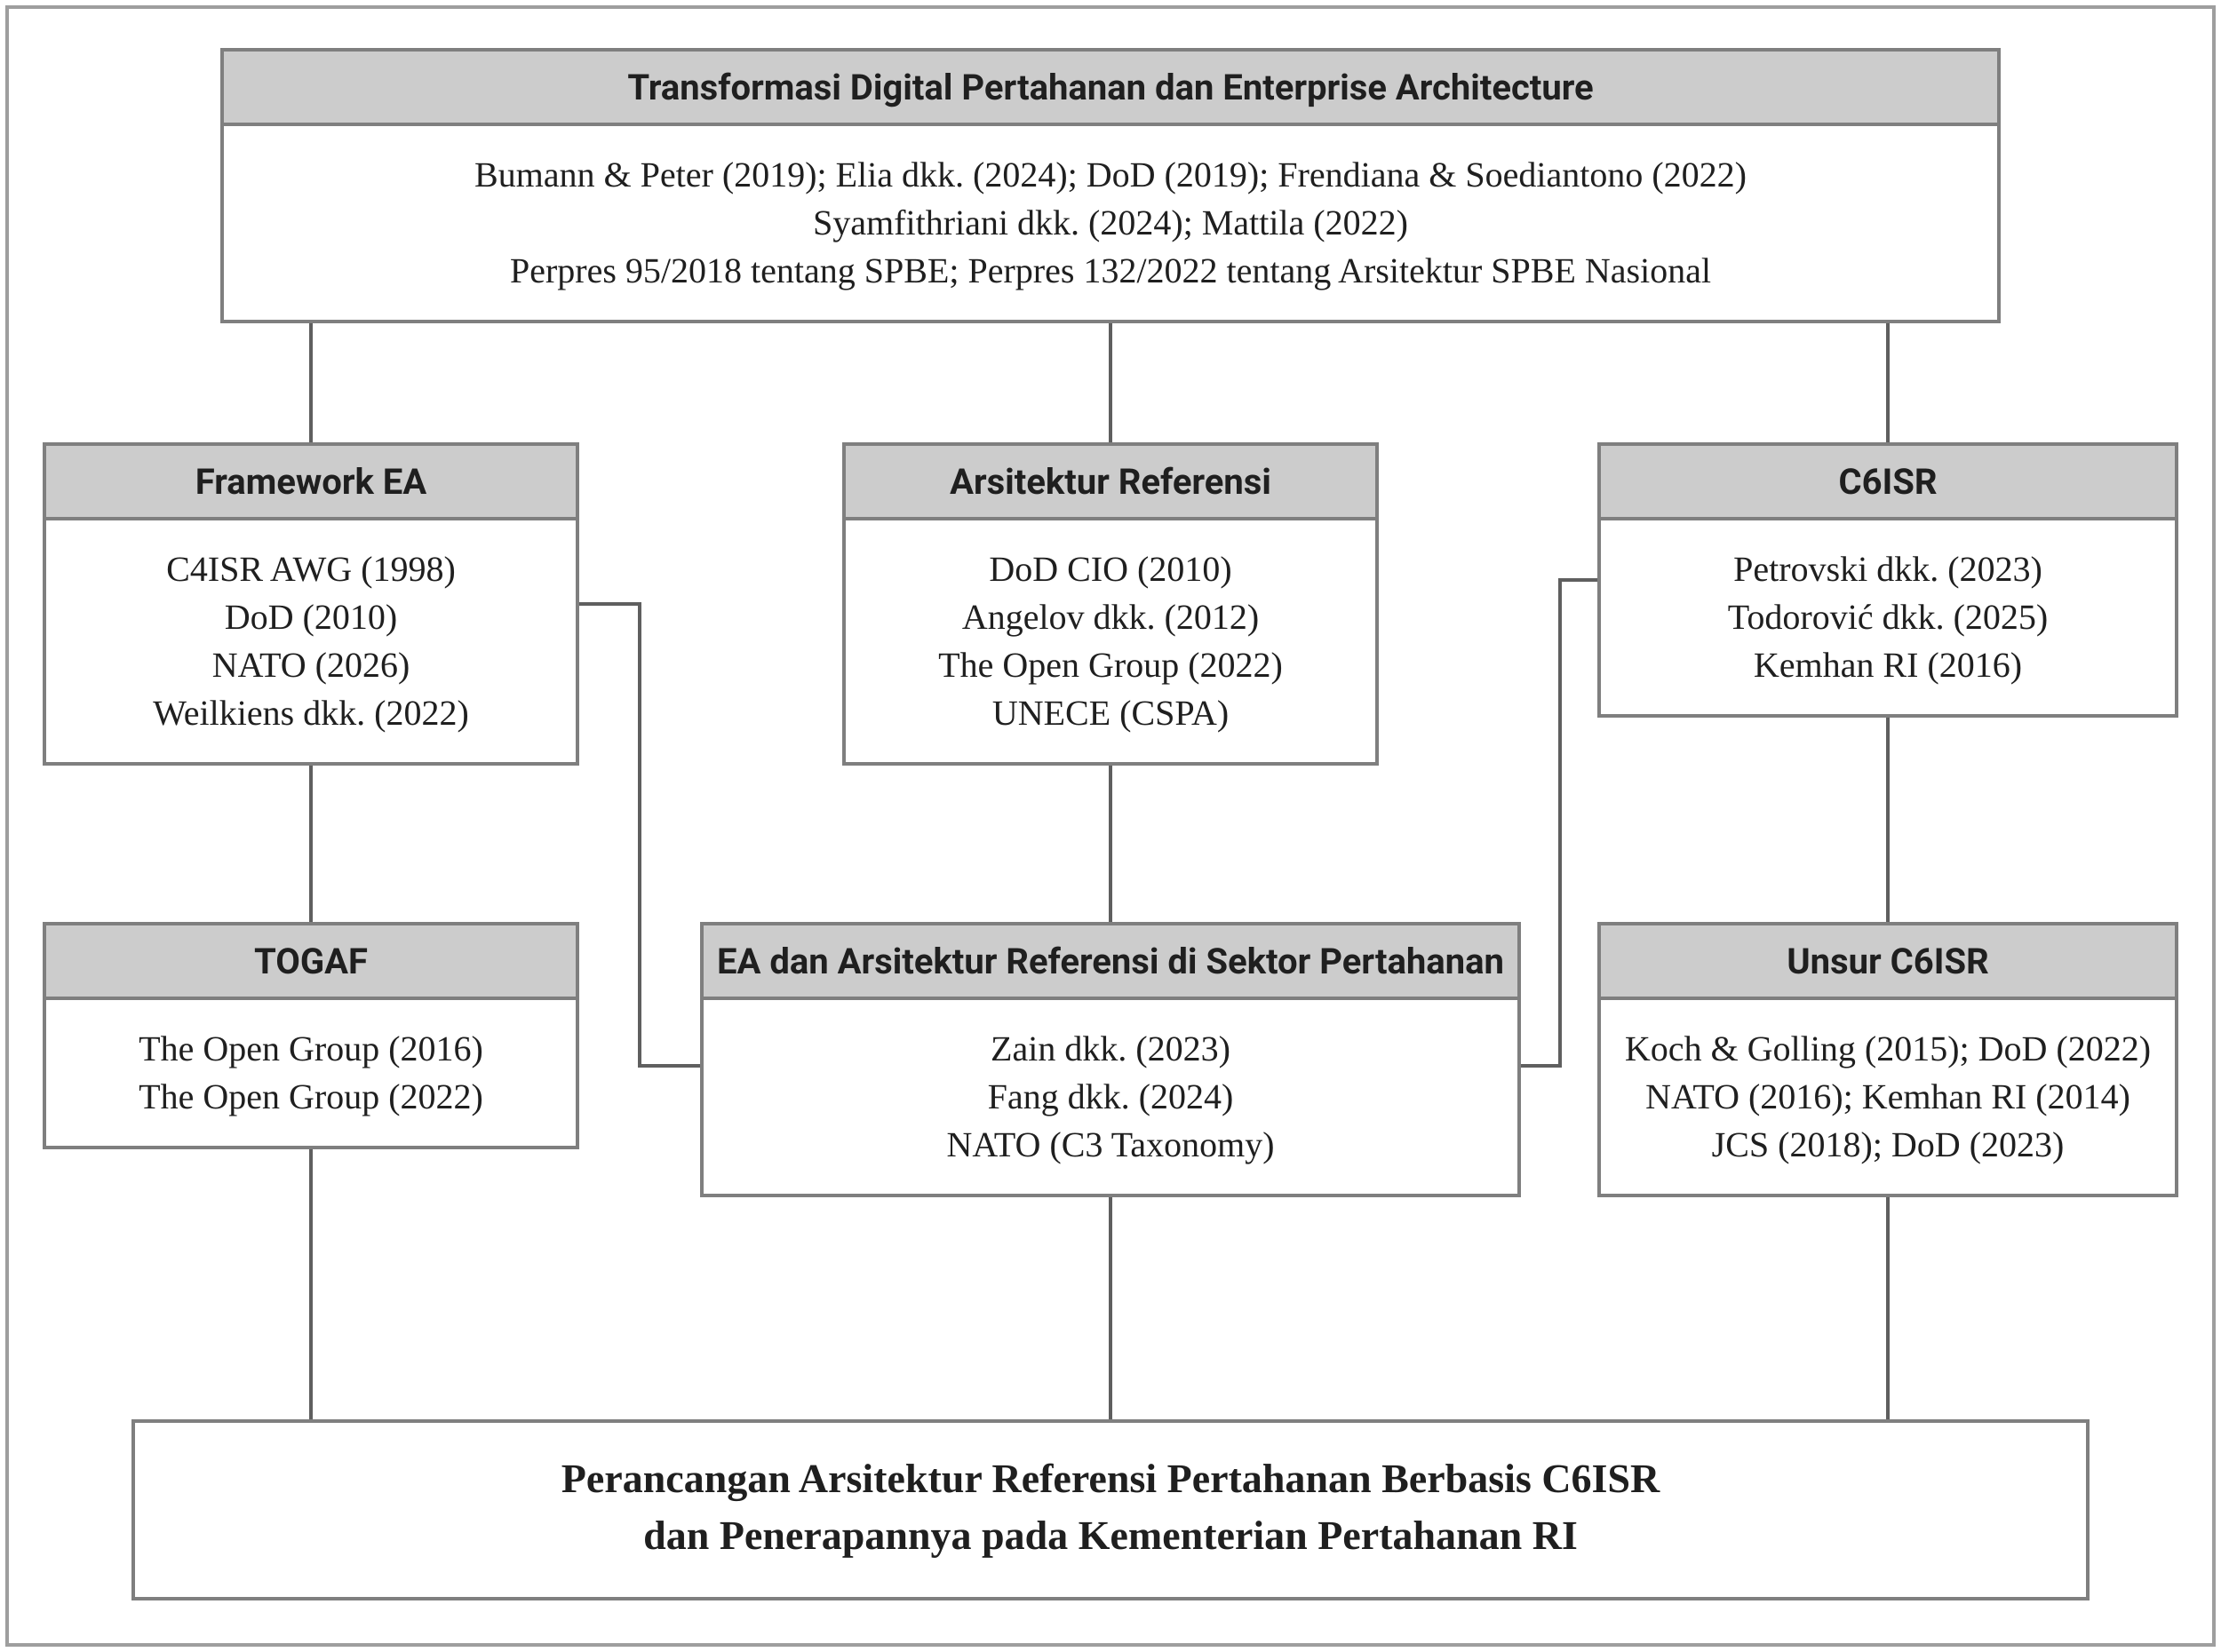
\includegraphics[width=1.00\linewidth,height=0.8\textheight,keepaspectratio]{images/Peta Literatur.png}
\caption{Peta Literatur}
\label{fig:II.1}
\end{figure}

Gambar~\ref{fig:II.1} menunjukkan bahwa peta literatur berangkat dari kajian transformasi digital pertahanan dan EA, termasuk Arsitektur SPBE sebagai EA pemerintah Indonesia. Kajian tersebut kemudian bercabang menjadi tiga. Cabang pertama membahas \textit{framework} EA hingga TOGAF, yang digunakan sebagai metode penerapan arsitektur referensi. Cabang kedua membahas konsep arsitektur referensi sebagai jenis artefak yang dirancang. Cabang ketiga membahas C6ISR beserta unsurnya sebagai landasan muatan pertahanan. Penelitian EA dan arsitektur referensi di sektor pertahanan menghubungkan ketiga cabang tersebut, dan seluruh cabang bermuara pada perancangan arsitektur referensi pertahanan berbasis C6ISR dalam penelitian ini.

\section{Transformasi Digital di Sektor Pertahanan}
\label{sec:II.2}

Subbab ini membahas konsep transformasi digital, praktiknya di sektor pertahanan, konsep pertahanan cerdas dan \textit{network centric warfare}, serta transformasi digital di Kemhan RI.

\subsection{Konsep Transformasi Digital}
\label{sec:II.2.1}

Transformasi digital adalah perubahan menyeluruh yang memanfaatkan teknologi digital untuk menciptakan nilai baru dan mengubah cara organisasi beroperasi. Berbeda dengan digitalisasi, transformasi digital tidak berhenti pada adopsi teknologi, tetapi juga mengubah proses bisnis, tata kelola, dan budaya organisasi.

\textcite{Bumann2019} mengidentifikasi enam bidang aksi transformasi digital, yaitu strategi, organisasi, budaya, teknologi, pelanggan, dan manusia, sebagaimana ditunjukkan pada Gambar~\ref{fig:II.2}. \textcite{Elia2024} memandang transformasi digital sebagai proses strategis yang menghubungkan kemampuan teknologi dengan kapabilitas organisasi, mulai dari tujuan, proses, mitra, manusia, dan platform, hingga perlindungan dan privasi data.

\begin{figure}[htbp]
\centering
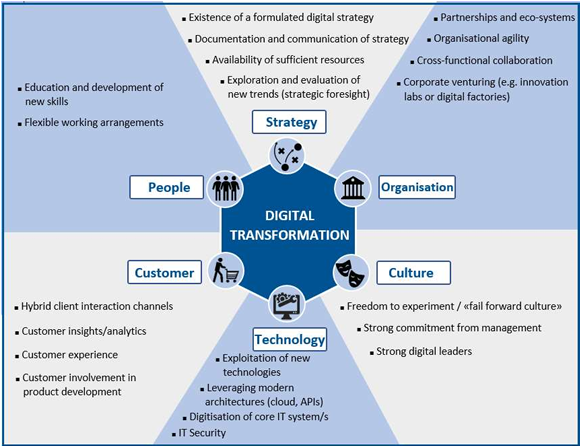
\includegraphics[width=0.79\linewidth,height=0.8\textheight,keepaspectratio]{images/Bidang Aksi Transformasi Digital.png}
\caption{Bidang Aksi Transformasi Digital}
\label{fig:II.2}
\end{figure}

Gambar~\ref{fig:II.2} menunjukkan bahwa teknologi hanya merupakan salah satu dari enam bidang aksi, sehingga transformasi digital membutuhkan keselarasan antara strategi, organisasi, manusia, dan teknologi. Di Indonesia, RPJPN 2025–2045 menetapkan transformasi digital sebagai agenda pembangunan nasional untuk membangun ekosistem digital yang tangguh dan berdaulat melalui penguatan infrastruktur digital, SDM\label{sk:SDM} digital, regulasi, integrasi data lintas sektor, serta riset dan inovasi \cite{UU59Tahun2024}.

\subsection{Praktik Transformasi Digital Pertahanan}
\label{sec:II.2.2}

Transformasi digital juga menjadi kebutuhan di sektor pertahanan, termasuk industri pertahanan \cite{Frendiana2022}. Dibandingkan sektor publik pada umumnya, transformasi digital pertahanan lebih kompleks karena mencakup pengelolaan informasi strategis, interoperabilitas sistem senjata, keamanan siber, dan dukungan operasi militer secara \textit{real-time}. Praktik di beberapa negara menunjukkan bahwa transformasi digital pertahanan dijalankan sebagai strategi nasional, antara lain sebagai berikut.

\begin{enumerate}[label=\arabic*.]
\item Amerika Serikat. \textit{DoD\label{sk:DoD} Digital Modernization Strategy} menetapkan empat prioritas, yaitu keamanan siber, kecerdasan buatan, \textit{cloud}, serta komando, kendali, dan komunikasi (C3). Prioritas tersebut dijabarkan ke dalam empat tujuan, yaitu inovasi untuk keunggulan kompetitif, optimalisasi efisiensi dan kapabilitas, penguatan keamanan siber, serta pengembangan talenta digital \cite{USDoD2019}, sebagaimana ditunjukkan pada Gambar~\ref{fig:II.3}.
\item Singapura. Strategi \textit{Total Defence} yang diperkenalkan sejak tahun 1984 memandang pertahanan sebagai tanggung jawab seluruh elemen bangsa. Pada tahun 2019, \textit{Digital Defence} ditambahkan sebagai pilar keenam untuk menghadapi ancaman dari ranah digital, melengkapi pilar \textit{Military}, \textit{Civil}, \textit{Economic}, \textit{Social}, dan \textit{Psychological Defence} \cite{MINDEF2019}, sebagaimana ditunjukkan pada Gambar~\ref{fig:II.4}.
\end{enumerate}

\begin{figure}[htbp]
\centering
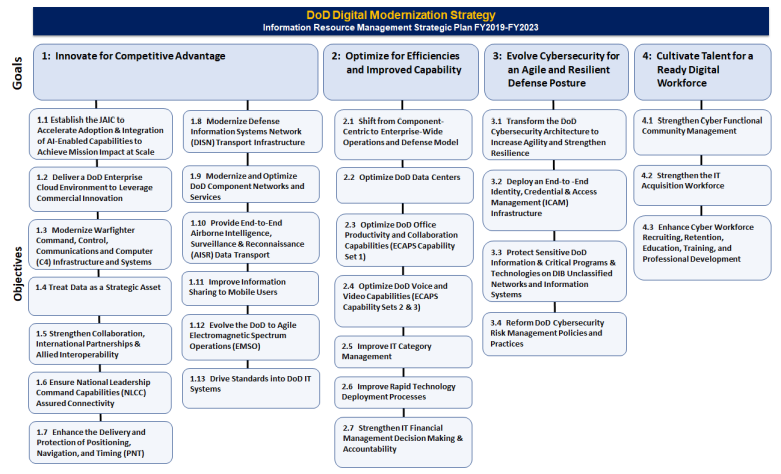
\includegraphics[width=1.00\linewidth,height=0.8\textheight,keepaspectratio]{images/DoD Digital Modernization Strategy.png}
\caption{\textit{DoD Digital Modernization Strategy}}
\label{fig:II.3}
\end{figure}

\begin{figure}[htbp]
\centering
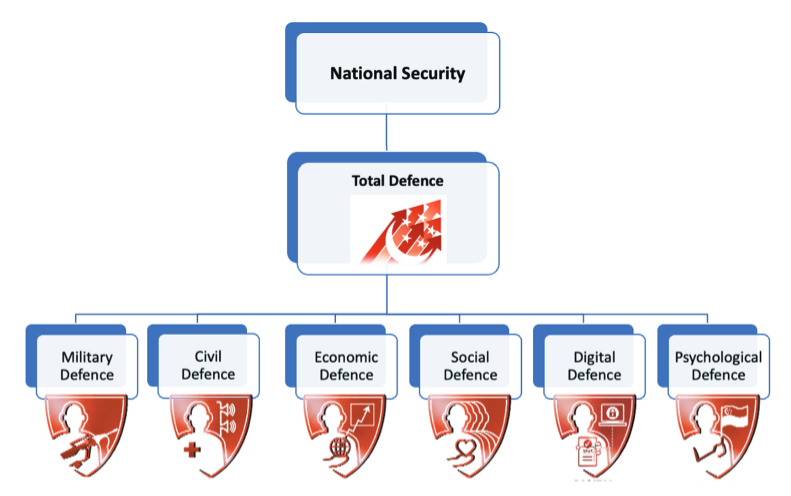
\includegraphics[width=0.79\linewidth,height=0.8\textheight,keepaspectratio]{images/Total Defence Singapura.png}
\caption{\textit{Total Defence} Singapura}
\label{fig:II.4}
\end{figure}

Gambar~\ref{fig:II.3} dan Gambar~\ref{fig:II.4} menunjukkan bahwa transformasi digital pertahanan tidak hanya menyangkut teknologi, tetapi juga keamanan siber, talenta digital, dan keterlibatan lintas organisasi.

\subsection{Pertahanan Cerdas dan Network Centric Warfare}
\label{sec:II.2.3}

Istilah \textit{smart defence} diperkenalkan NATO pada KTT\label{sk:KTT} Chicago 2012 sebagai pendekatan pengembangan kapabilitas melalui prioritisasi, spesialisasi, dan kerja sama multinasional \cite{NATO2012Forces2020}. Dalam penelitian ini, pertahanan cerdas dimaknai lebih luas sebagai pemanfaatan teknologi digital, data, dan sistem terintegrasi untuk meningkatkan efektivitas pertahanan. Dalam paradigma ini, data diposisikan sebagai aset strategis, dan keunggulan informasi (\textit{information superiority}) menjadi penentu keunggulan operasi \cite{Koch2015}.

Konsep yang mendasari pertahanan cerdas adalah \textit{network centric warfare} (NCW\label{sk:NCW}). NCW menekankan bahwa kekuatan tempur berasal dari kemampuan menghubungkan sensor, komando dan kendali, unit tempur, dan pengambil keputusan dalam satu jaringan informasi, sehingga informasi dapat dibagikan secara \textit{real-time} \cite{Koch2015}. Gambar~\ref{fig:II.5} menunjukkan arsitektur NCW yang terdiri atas lapisan darat, udara, dan antariksa. Setiap simpul dapat bertukar data melalui beberapa jalur alternatif, sehingga jaringan tetap berfungsi meskipun sebagian simpul terganggu.

\begin{figure}[htbp]
\centering
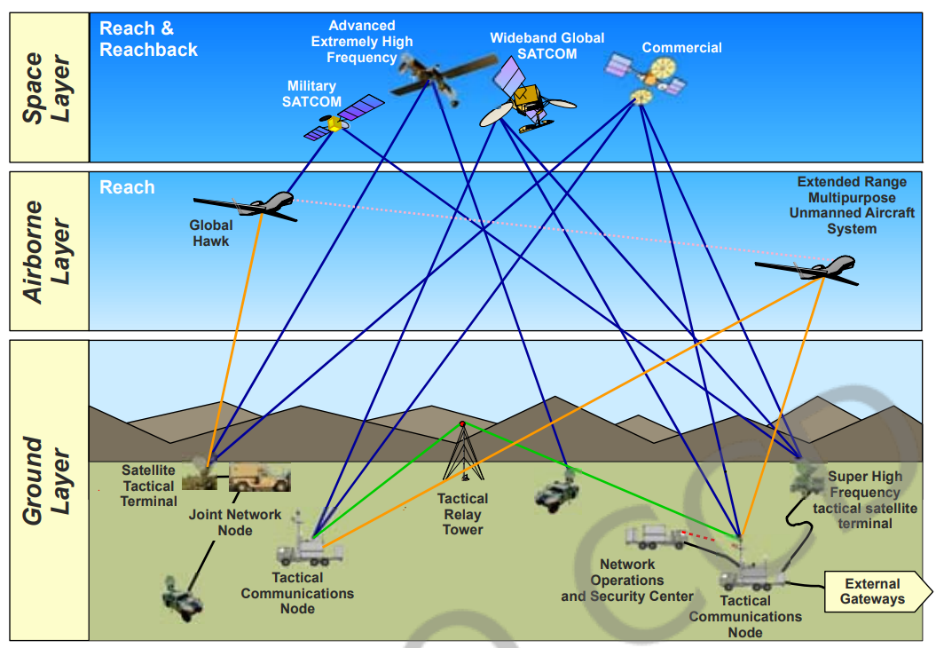
\includegraphics[width=0.93\linewidth,height=0.8\textheight,keepaspectratio]{images/Arsitektur Network Centric Warfare.png}
\caption{Arsitektur \textit{Network Centric Warfare}}
\label{fig:II.5}
\end{figure}

NCW kemudian berkembang menjadi \textit{Joint All-Domain Command and Control} (JADC2\label{sk:JADC2}), yaitu strategi Departemen Pertahanan Amerika Serikat untuk mengintegrasikan komando dan kendali lintas domain darat, laut, udara, antariksa, dan siber \cite{USDoD2022}. JADC2 dibangun atas tiga fungsi, yaitu \textit{sense} (mengumpulkan dan membagikan data dari seluruh domain), \textit{make sense} (mengolah data menjadi pemahaman situasi), dan \textit{act} (mengambil serta mendistribusikan keputusan secara cepat dan aman), sebagaimana ditunjukkan pada Gambar~\ref{fig:II.6}.

\begin{figure}[htbp]
\centering
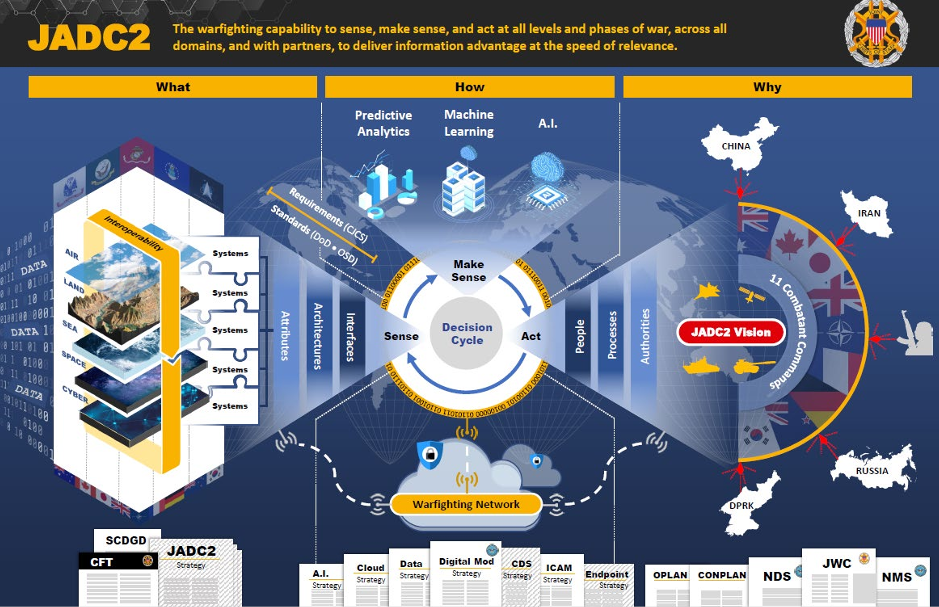
\includegraphics[width=1.00\linewidth,height=0.8\textheight,keepaspectratio]{images/Strategi Joint All-Domain Command and Control (JADC2).png}
\caption{Strategi \textit{Joint All-Domain Command and Control} (JADC2)}
\label{fig:II.6}
\end{figure}

Gambar~\ref{fig:II.5} dan Gambar~\ref{fig:II.6} menunjukkan bahwa keunggulan pertahanan modern bergantung pada integrasi data, interoperabilitas, dan keamanan jaringan lintas organisasi. Integrasi lintas organisasi tersebut tidak dapat dicapai apabila setiap organisasi pertahanan membangun arsitekturnya sendiri-sendiri, sehingga dibutuhkan acuan arsitektur bersama.

\subsection{Transformasi Digital Kemhan RI}
\label{sec:II.2.4}

Transformasi digital Kemhan RI merupakan bagian dari modernisasi pertahanan sekaligus pembenahan tata kelola pemerintahan. Landasan kebijakan transformasi digital Kemhan RI adalah sebagai berikut.

\begin{enumerate}[label=\arabic*.]
\item Sistem Pemerintahan Berbasis Elektronik (SPBE). Perpres\label{sk:Perpres} Nomor 95 Tahun 2018 mewajibkan setiap instansi pusat menyusun Arsitektur SPBE dan Peta Rencana SPBE untuk jangka waktu lima tahun \cite{Perpres95Tahun2018}, dengan berpedoman pada Arsitektur SPBE Nasional \cite{Perpres132Tahun2022}.
\item Percepatan transformasi digital. Perpres Nomor 82 Tahun 2023 mendorong keterpaduan layanan digital nasional, antara lain melalui aplikasi SPBE prioritas yang digunakan bersama oleh instansi pemerintah \cite{Perpres82Tahun2023}. Upaya tersebut diperkuat dengan pembentukan Komite Percepatan Transformasi Digital Pemerintah \cite{Perpres83Tahun2025}.
\item Tata kelola data. Permenhan\label{sk:Permenhan} Nomor 1 Tahun 2023 menjabarkan kebijakan Satu Data Indonesia di sektor pertahanan, termasuk penyelenggara Satu Data Pertahanan serta Portal Satu Data Pertahanan sebagai media bagi pakai data \cite{Permenhan1Tahun2023}.
\item Keamanan siber. Pedoman Pertahanan Siber menjadi acuan dalam menghadapi ancaman terhadap perangkat keras, perangkat lunak, serta data dan informasi pertahanan \cite{Permenhan82Tahun2014}. Pelindungan infrastruktur informasi vital sektor pertahanan juga telah memiliki peta jalan untuk tahun 2025–2029 \cite{Permenhan34Tahun2025}.
\end{enumerate}

Secara kelembagaan, pengelolaan data, sistem informasi, dan infrastruktur TIK\label{sk:TIK} merupakan tugas Pusat Data dan Informasi (Pusdatin\label{sk:Pusdatin}) \cite{Permenhan30Tahun2025}, yang juga berperan sebagai Walidata Satu Data Pertahanan \cite{Pusdatin2026SatuData}. Pelaksanaan kebijakan tersebut telah menunjukkan sejumlah capaian. Indeks SPBE Kemhan RI meningkat dari 2,62 pada tahun 2022 menjadi 3,43 pada tahun 2023 dengan predikat Baik \cite{Pusdatin2024}. Indeks Satu Data Indonesia Kemhan RI tahun 2025 mencapai 81,35, di atas rata-rata nasional tahun 2024 sebesar 51,07 \cite{Pusdatin2026SatuData}. Kemhan RI juga mulai mengintegrasikan layanan digitalnya melalui \textit{Single Sign-On} (SSO\label{sk:SSO}) yang menghubungkan berbagai aplikasi satuan kerja melalui satu identitas pengguna \cite{Pusdatin2026SSO}.

Meskipun demikian, capaian tersebut masih bersifat parsial. Evaluasi Satu Data Pertahanan tahun 2026 menunjukkan bahwa Indeks Pembangunan Statistik Kemhan RI tahun 2024 masih berpredikat Cukup dengan nilai 2,14, sedangkan pengelolaan informasi geospasial tahun 2025 baru berada pada tingkat Operasional dengan nilai 2,54. Evaluasi tersebut juga mengidentifikasi empat kendala utama, yaitu kelembagaan dan koordinasi, kualitas data, integrasi sistem, serta kapasitas SDM \cite{Pusdatin2026SatuData}. Tantangan transformasi digital Kemhan RI dirangkum per dimensi pada Tabel~\ref{tab:II.1}.

\begingroup\small\setstretch{1.0}
\begin{longtable}{@{}>{\raggedright\arraybackslash\hspace{0pt}}p{0.069\linewidth}>{\raggedright\arraybackslash\hspace{0pt}}p{0.154\linewidth}>{\raggedright\arraybackslash\hspace{0pt}}p{0.375\linewidth}>{\raggedright\arraybackslash\hspace{0pt}}p{0.309\linewidth}@{}}
\caption{Tantangan Transformasi Digital Kemhan RI}\label{tab:II.1}\\
\toprule
\textbf{No.} & \textbf{Dimensi} & \textbf{Kondisi Saat Ini} & \textbf{Dampak}\\
\midrule
\endfirsthead
\multicolumn{4}{@{}l}{\small\itshape \tablename\ \thetable{} (lanjutan)}\\
\toprule
\textbf{No.} & \textbf{Dimensi} & \textbf{Kondisi Saat Ini} & \textbf{Dampak}\\
\midrule
\endhead
\bottomrule
\endlastfoot
\centering\arraybackslash 1 & Tata kelola & Pusdatin berperan menjalankan sistem yang sudah ada, dan belum ada fungsi yang mengorkestrasi transformasi lintas satuan kerja dan matra. & Perencanaan dan pengembangan sistem berjalan sendiri-sendiri per satuan kerja.\\*
\centering\arraybackslash 2 & Data & Data terkotak per aplikasi. Kamus data, klasifikasi data, dan kanal berbagi pakai belum tersedia, serta kualitas data dan statistik sektoral belum optimal. & Data sulit dibagi pakai dan dianalisis lintas domain.\\
\centering\arraybackslash 3 & Aplikasi & Terdapat 247 aplikasi (176 umum dan 71 khusus). Sebagian aplikasi khusus memiliki fungsi serupa dan mekanisme autentikasi yang berbeda. & Investasi berulang dan integrasi antaraplikasi sulit dilakukan.\\
\centering\arraybackslash 4 & Teknologi & Seluruh layanan bertumpu pada satu \textit{data center} tanpa \textit{disaster recovery center}. & Terdapat titik tunggal kegagalan (\textit{single point of failure}).\\
\centering\arraybackslash 5 & Keamanan siber & Pengamanan masih parsial, sedangkan konektivitas yang makin tinggi memperbesar dampak intrusi. & Layanan dan data pertahanan rentan terhadap gangguan dan serangan siber.\\
\centering\arraybackslash 6 & SDM & Kompetensi digital, statistik, dan geospasial belum merata. & Kualitas implementasi bergantung pada kemampuan masing-masing unit.\\*
\centering\arraybackslash 7 & Operasional & Komando dan kendali dikembangkan per matra, dan sistem dengan standar berbeda sulit bertukar informasi. & Keterpaduan ISR, komando-kendali, dan unsur penindak dalam operasi gabungan sulit dicapai.\\
\end{longtable}
\endgroup

Tabel~\ref{tab:II.1} menunjukkan bahwa tantangan transformasi digital Kemhan RI saling terkait dan mencakup seluruh lapisan, mulai dari tata kelola hingga operasional. Tantangan pada dimensi operasional juga melibatkan Mabes TNI dan ketiga matra, sehingga tidak dapat diselesaikan oleh Kemhan RI secara sendiri. Oleh karena itu, transformasi digital pertahanan membutuhkan acuan arsitektur bersama yang menautkan strategi dengan proses bisnis, data, aplikasi, teknologi, dan kapabilitas operasional lintas organisasi pertahanan.

\section{Enterprise Architecture}
\label{sec:II.3}

Subbab ini membahas konsep dan domain EA, manfaat EA dalam transformasi digital, serta Arsitektur SPBE sebagai EA pemerintah Indonesia.

\subsection{Konsep dan Domain Enterprise Architecture}
\label{sec:II.3.1}

Istilah \textit{Enterprise Architecture} (EA) tersusun atas dua konsep, yaitu \textit{enterprise} dan arsitektur. TOGAF memandang \textit{enterprise} sebagai kumpulan organisasi yang memiliki tujuan bersama, sehingga \textit{enterprise} dapat berupa satu kementerian beserta seluruh satuan kerjanya. Adapun arsitektur adalah konsep atau sifat fundamental suatu sistem yang diwujudkan dalam elemen-elemennya, hubungan antarelemen, serta prinsip perancangan dan evolusinya \cite{TOGAF2022}.

Lankhorst mendefinisikan EA sebagai satu kesatuan prinsip, metode, dan model yang koheren untuk merancang dan mewujudkan struktur organisasi, proses bisnis, sistem informasi, dan infrastruktur suatu \textit{enterprise} \cite{Lankhorst2017}. Ross dkk. memandang EA sebagai logika pengorganisasian (\textit{organizing logic}) proses bisnis dan infrastruktur TI\label{sk:TI} yang mencerminkan kebutuhan integrasi dan standardisasi model operasi organisasi \cite{Ross2006}. Kedua definisi tersebut menunjukkan bahwa EA tidak hanya menyangkut teknologi, tetapi juga keterpaduan seluruh komponen organisasi.

EA mendeskripsikan kondisi saat ini (\textit{baseline}), kondisi yang diinginkan (\textit{target}), serta \textit{roadmap} untuk berpindah di antara keduanya \cite{Tamm2011}. TOGAF membagi EA ke dalam empat domain utama, yaitu bisnis, data, aplikasi, dan teknologi, dengan arsitektur data dan aplikasi secara bersama-sama disebut arsitektur sistem informasi \cite{TOGAF2022}. Hubungan antardomain dan antarkondisi tersebut ditunjukkan pada Gambar~\ref{fig:II.7}.

\begin{figure}[htbp]
\centering
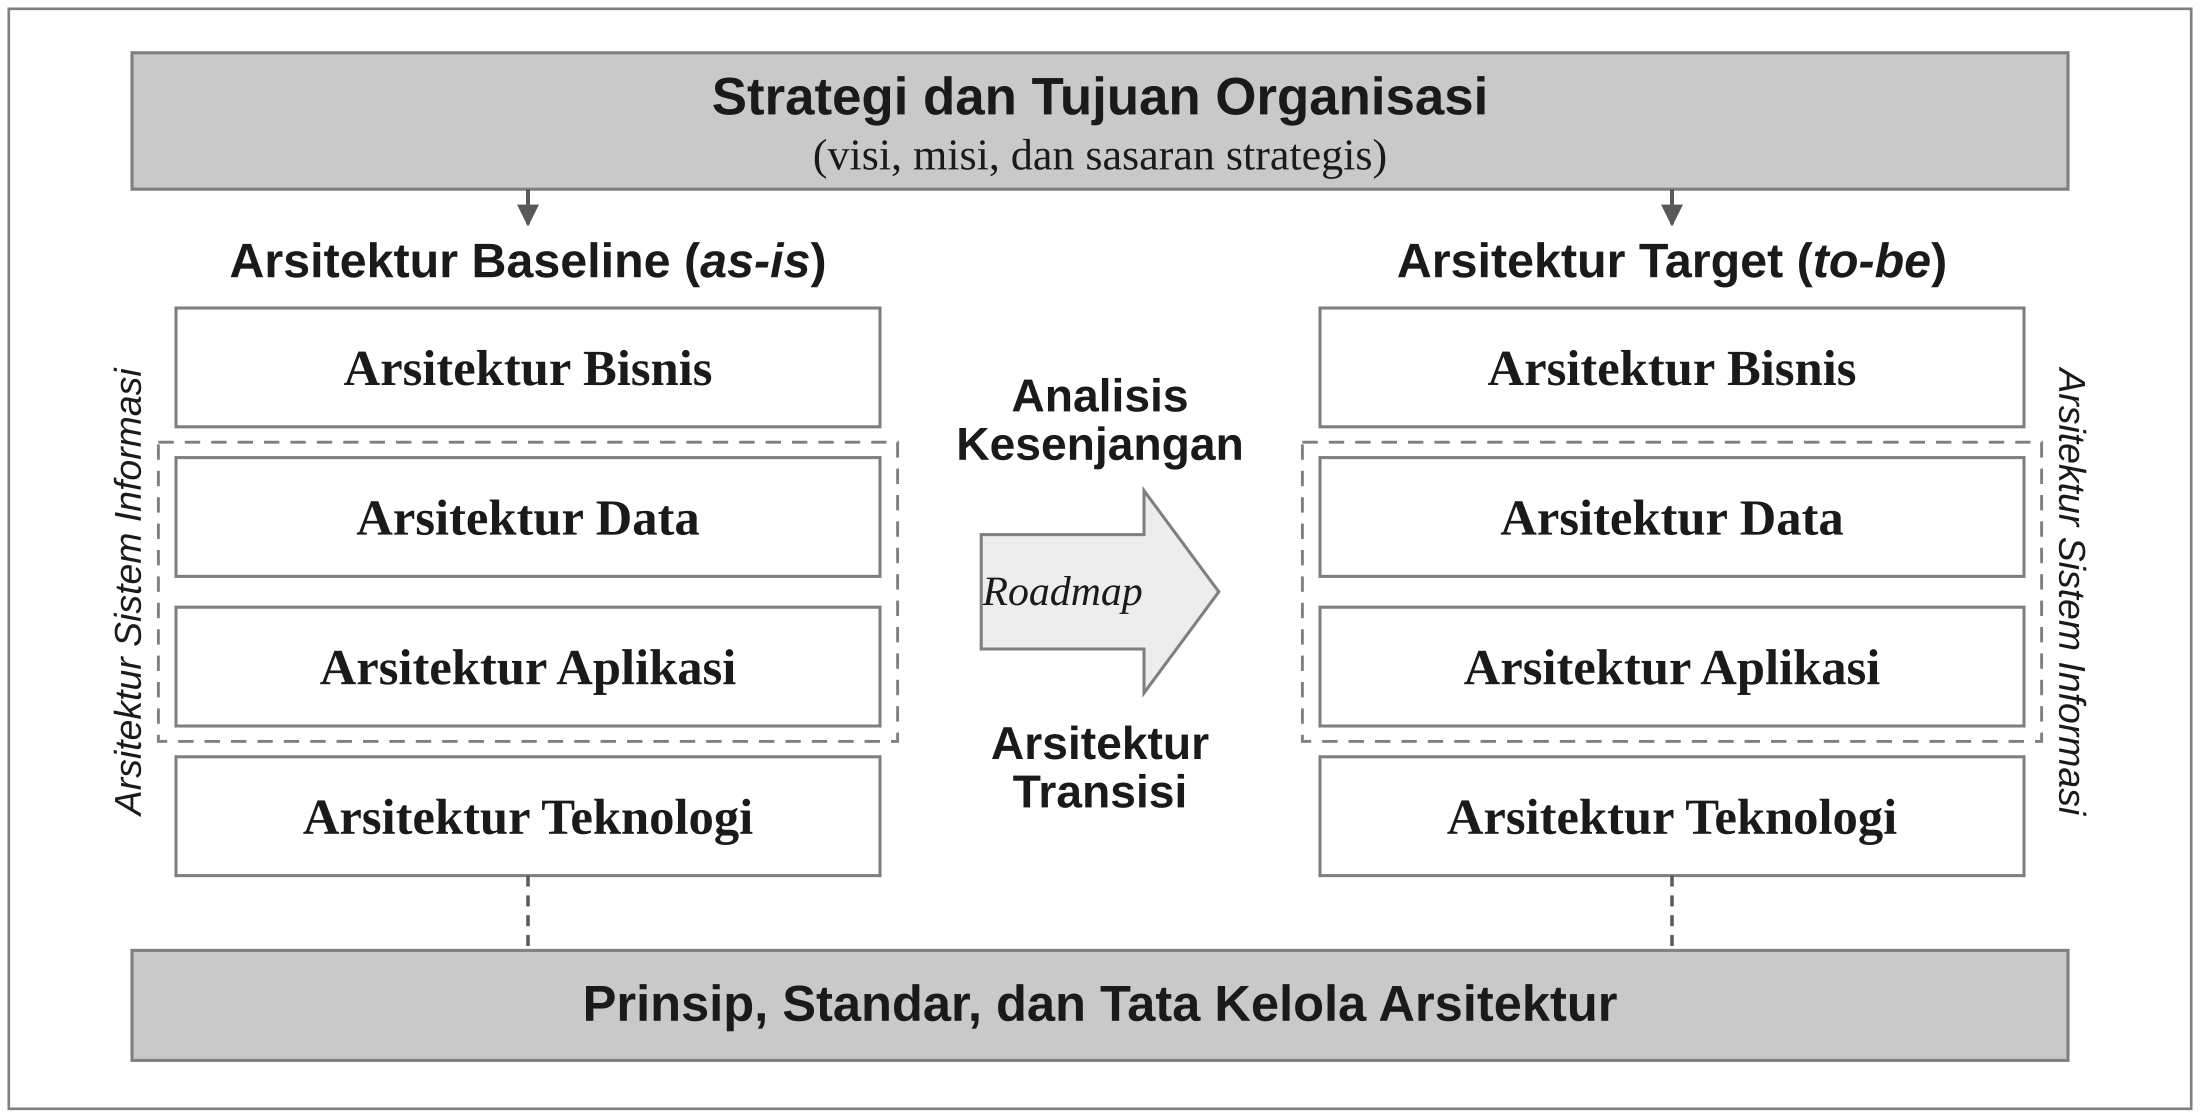
\includegraphics[width=1.00\linewidth,height=0.8\textheight,keepaspectratio]{images/Domain dan Kondisi Arsitektur dalam EA.png}
\caption{Domain dan Kondisi Arsitektur dalam EA}
\label{fig:II.7}
\end{figure}

Gambar~\ref{fig:II.7} menunjukkan bahwa strategi dan tujuan organisasi mengarahkan seluruh domain arsitektur. Arsitektur bisnis mendeskripsikan strategi, tata kelola, organisasi, dan proses bisnis. Arsitektur data mendeskripsikan struktur aset data dan pengelolaannya. Arsitektur aplikasi mendeskripsikan aplikasi yang mendukung proses bisnis beserta interaksinya. Arsitektur teknologi mendeskripsikan perangkat keras, perangkat lunak, dan jaringan yang menopang ketiga domain lainnya \cite{TOGAF2022}. Kesenjangan antara kondisi \textit{baseline} dan \textit{target} pada setiap domain menjadi dasar penyusunan \textit{roadmap}, sedangkan konsistensi seluruh rancangan dijaga oleh prinsip, standar, dan tata kelola arsitektur.

Dalam penelitian ini, EA dimaknai sebagai rancangan menyeluruh yang menyelaraskan strategi organisasi pertahanan dengan proses bisnis, data, aplikasi, dan teknologi, beserta \textit{roadmap} untuk mewujudkannya. Kapabilitas operasional C6ISR tidak ditambahkan sebagai domain baru, tetapi diterjemahkan ke dalam keempat domain tersebut melalui arsitektur referensi.

\subsection{Manfaat EA dalam Transformasi Digital}
\label{sec:II.3.2}

Transformasi digital menuntut perubahan serentak pada strategi, proses bisnis, data, dan teknologi. Tanpa acuan bersama, perubahan tersebut berisiko berjalan sendiri-sendiri dan justru menambah kompleksitas. Kajian literatur sistematis oleh Syamfithriani dkk. menunjukkan bahwa EA berperan penting dalam transformasi digital, terutama dalam merancang dan mengelola infrastruktur TI untuk menekan risiko dan kompleksitas \cite{Syamfithriani2024}. Tamm dkk. menjelaskan bahwa EA memberikan nilai melalui empat manfaat (\textit{benefit enablers}) berikut \cite{Tamm2011}.

\begin{enumerate}[label=\arabic*.]
\item Keselarasan organisasi (\textit{organisational alignment}), yaitu keselarasan antara strategi organisasi dan TI.
\item Ketersediaan informasi (\textit{information availability}), yaitu tersedianya informasi yang berkualitas dan konsisten bagi pengambil keputusan.
\item Optimalisasi portofolio sumber daya (\textit{resource portfolio optimisation}), yaitu pengelolaan portofolio aplikasi dan infrastruktur secara efisien, termasuk mengurangi duplikasi.
\item Komplementaritas sumber daya (\textit{resource complementarity}), yaitu kemampuan berbagai sumber daya TI untuk saling melengkapi dan bekerja bersama.
\end{enumerate}

EA juga memandang transformasi sebagai proses bertahap. Ross dkk. mengidentifikasi empat tahap kematangan arsitektur, yaitu \textit{business silos}, \textit{standardized technology}, \textit{optimized core}, dan \textit{business modularity} \cite{Ross2006}, sebagaimana ditunjukkan pada Gambar~\ref{fig:II.8}.

\begin{figure}[htbp]
\centering
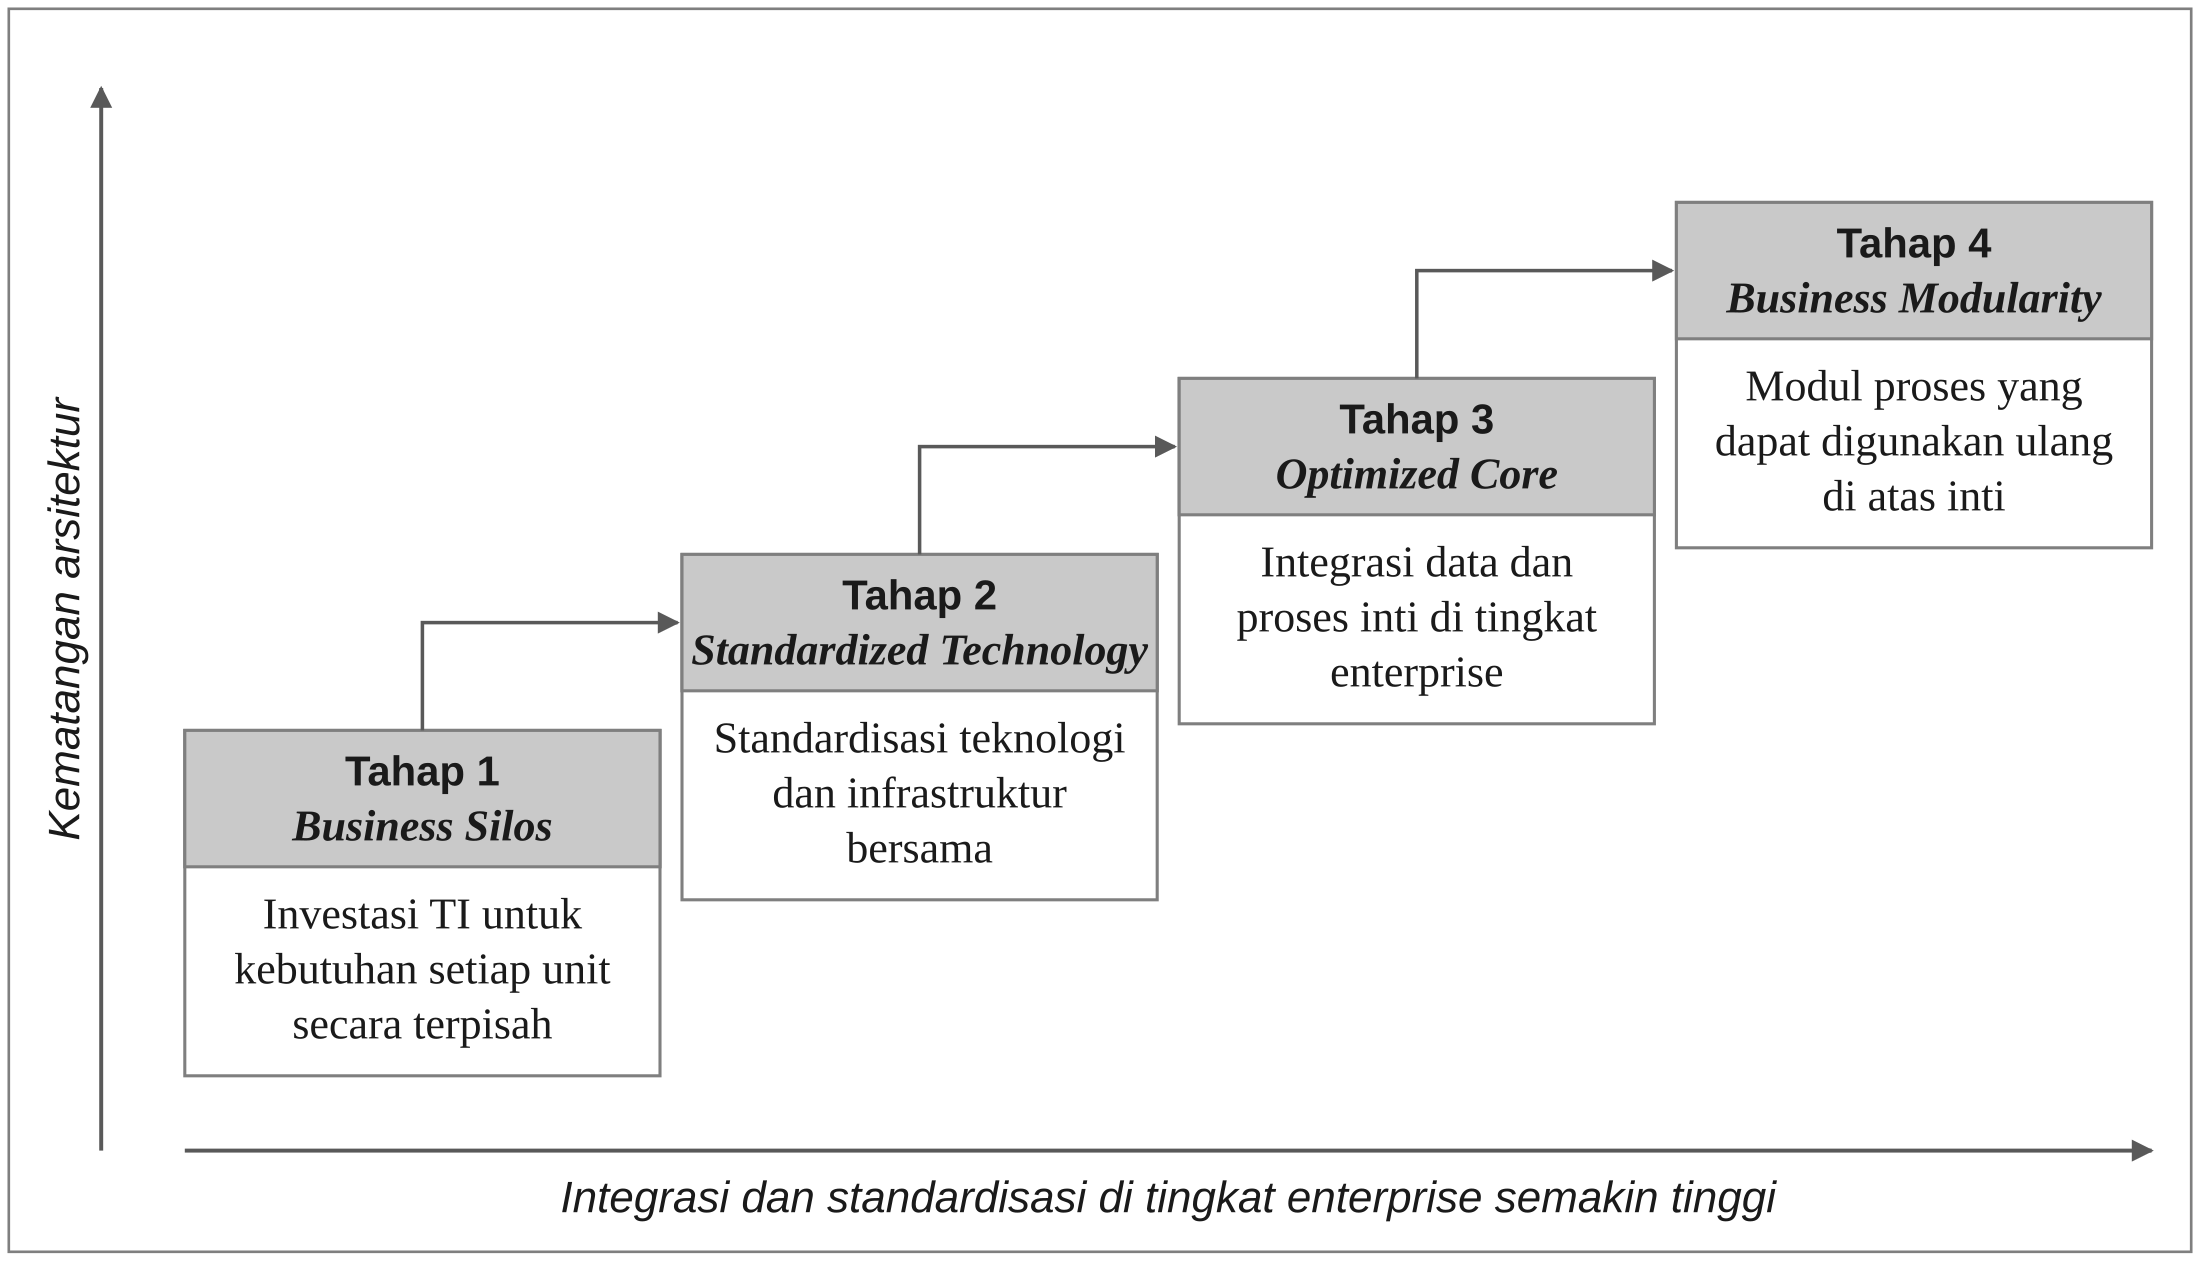
\includegraphics[width=1.00\linewidth,height=0.8\textheight,keepaspectratio]{images/Tahap Kematangan Arsitektur Menurut Ross dkk.png}
\caption{Tahap Kematangan Arsitektur Menurut Ross dkk.}
\label{fig:II.8}
\end{figure}

Gambar~\ref{fig:II.8} menunjukkan bahwa pada tahap \textit{business silos}, investasi TI ditujukan untuk kebutuhan setiap unit secara terpisah. Tahap \textit{standardized technology} menstandarkan teknologi bersama, tahap \textit{optimized core} mengintegrasikan data dan proses inti di tingkat \textit{enterprise}, dan tahap \textit{business modularity} menyusun modul proses yang dapat digunakan ulang di atas inti tersebut \cite{Ross2006}. Kondisi pada Tabel~\ref{tab:II.1} memiliki karakteristik tahap \textit{business silos}. Pada organisasi militer, Mattila menemukan bahwa metode tata kelola TIK yang umum belum menjawab seluruh permasalahan transformasi militer \cite{Mattila2022}, sehingga EA beserta \textit{framework} pendukungnya perlu disesuaikan dengan karakteristik organisasi pertahanan.

\subsection{Arsitektur SPBE sebagai EA Pemerintah Indonesia}
\label{sec:II.3.3}

Di Indonesia, penerapan EA pada instansi pemerintah diwujudkan melalui Arsitektur SPBE, yaitu kerangka dasar yang mendeskripsikan integrasi proses bisnis, data dan informasi, infrastruktur SPBE, aplikasi SPBE, dan keamanan SPBE untuk menghasilkan layanan SPBE yang terintegrasi. Arsitektur SPBE terdiri atas Arsitektur SPBE Nasional, Arsitektur SPBE Instansi Pusat, dan Arsitektur SPBE Pemerintah Daerah. Arsitektur SPBE Instansi Pusat disusun dengan berpedoman pada Arsitektur SPBE Nasional dan rencana strategis instansi untuk jangka waktu lima tahun \cite{Perpres95Tahun2018}.

Arsitektur SPBE Nasional ditetapkan melalui Perpres Nomor 132 Tahun 2022 dan memuat arah kebijakan dan strategi, kerangka kerja, referensi arsitektur, domain arsitektur, serta inisiatif strategis. Referensi arsitektur berisi komponen dasar arsitektur yang baku sebagai acuan, sedangkan domain arsitektur berisi substansi arsitektur. Keduanya mencakup enam domain, yaitu proses bisnis, data dan informasi, layanan, aplikasi, infrastruktur, dan keamanan \cite{Perpres132Tahun2022}. Padanan keenam domain tersebut dengan domain TOGAF ditunjukkan pada Tabel~\ref{tab:II.2}.

\begingroup\small\setstretch{1.0}
\begin{longtable}{@{}>{\raggedright\arraybackslash\hspace{0pt}}p{0.236\linewidth}>{\raggedright\arraybackslash\hspace{0pt}}p{0.406\linewidth}>{\raggedright\arraybackslash\hspace{0pt}}p{0.296\linewidth}@{}}
\caption{Pemetaan Domain Arsitektur SPBE dan Domain TOGAF}\label{tab:II.2}\\
\toprule
\textbf{Domain Arsitektur SPBE} & \textbf{Cakupan} & \textbf{Padanan pada TOGAF}\\
\midrule
\endfirsthead
\multicolumn{3}{@{}l}{\small\itshape \tablename\ \thetable{} (lanjutan)}\\
\toprule
\textbf{Domain Arsitektur SPBE} & \textbf{Cakupan} & \textbf{Padanan pada TOGAF}\\
\midrule
\endhead
\bottomrule
\endlastfoot
Proses Bisnis & Fungsi dan proses penyelenggaraan pemerintahan & \textit{Business Architecture}\\*
Layanan & Layanan administrasi pemerintahan dan layanan publik berbasis elektronik & \textit{Business Architecture} (layanan bisnis)\\
Data dan Informasi & Data dan informasi yang digunakan dan dihasilkan oleh proses bisnis & \textit{Data Architecture}\\
Aplikasi & Aplikasi yang mendukung proses bisnis dan layanan & \textit{Application Architecture}\\
Infrastruktur & Pusat data, jaringan intra, dan sistem penghubung layanan & \textit{Technology Architecture}\\*
Keamanan & Pengamanan data, aplikasi, dan infrastruktur & \textit{Security Architecture} (lintas domain)\\
\end{longtable}
\endgroup

Tabel~\ref{tab:II.2} menunjukkan bahwa domain Arsitektur SPBE selaras dengan domain TOGAF. Perbedaannya, keamanan ditetapkan sebagai domain tersendiri dalam Arsitektur SPBE, sedangkan TOGAF memperlakukannya sebagai \textit{concern} lintas domain \cite{TOGAFRiskSecurity}. Arsitektur SPBE juga menunjukkan bahwa mekanisme arsitektur referensi telah digunakan dalam pemerintahan Indonesia, yaitu arsitektur instansi disusun dengan mengacu pada referensi arsitektur nasional. Namun, referensi tersebut berorientasi pada layanan pemerintahan dan tidak memuat kapabilitas operasional pertahanan.

\section{TOGAF}
\label{sec:II.4}

\textit{The Open Group Architecture Framework} (TOGAF) merupakan standar EA yang dikembangkan oleh The Open Group. Versi pertamanya diterbitkan pada tahun 1995 dengan dasar \textit{Technical Architecture Framework for Information Management} (TAFIM\label{sk:TAFIM}) milik Departemen Pertahanan Amerika Serikat, sedangkan versi terkininya adalah \textit{TOGAF Standard, 10th Edition} yang dirilis pada tahun 2022. TOGAF digunakan oleh organisasi komersial, instansi pemerintah, hingga lembaga pertahanan \cite{TOGAF2022}.

\subsection{Struktur dan Komponen TOGAF}
\label{sec:II.4.1}

TOGAF 10 memisahkan konsep yang bersifat universal dari panduan yang bersifat rinci. Oleh karena itu, TOGAF dibagi menjadi \textit{TOGAF Fundamental Content} yang memuat konsep dan praktik inti, serta \textit{TOGAF Series Guides} yang memberikan panduan untuk kebutuhan tertentu \cite{TOGAF2022}, sebagaimana ditunjukkan pada Gambar~\ref{fig:II.9}.

\begin{figure}[htbp]
\centering
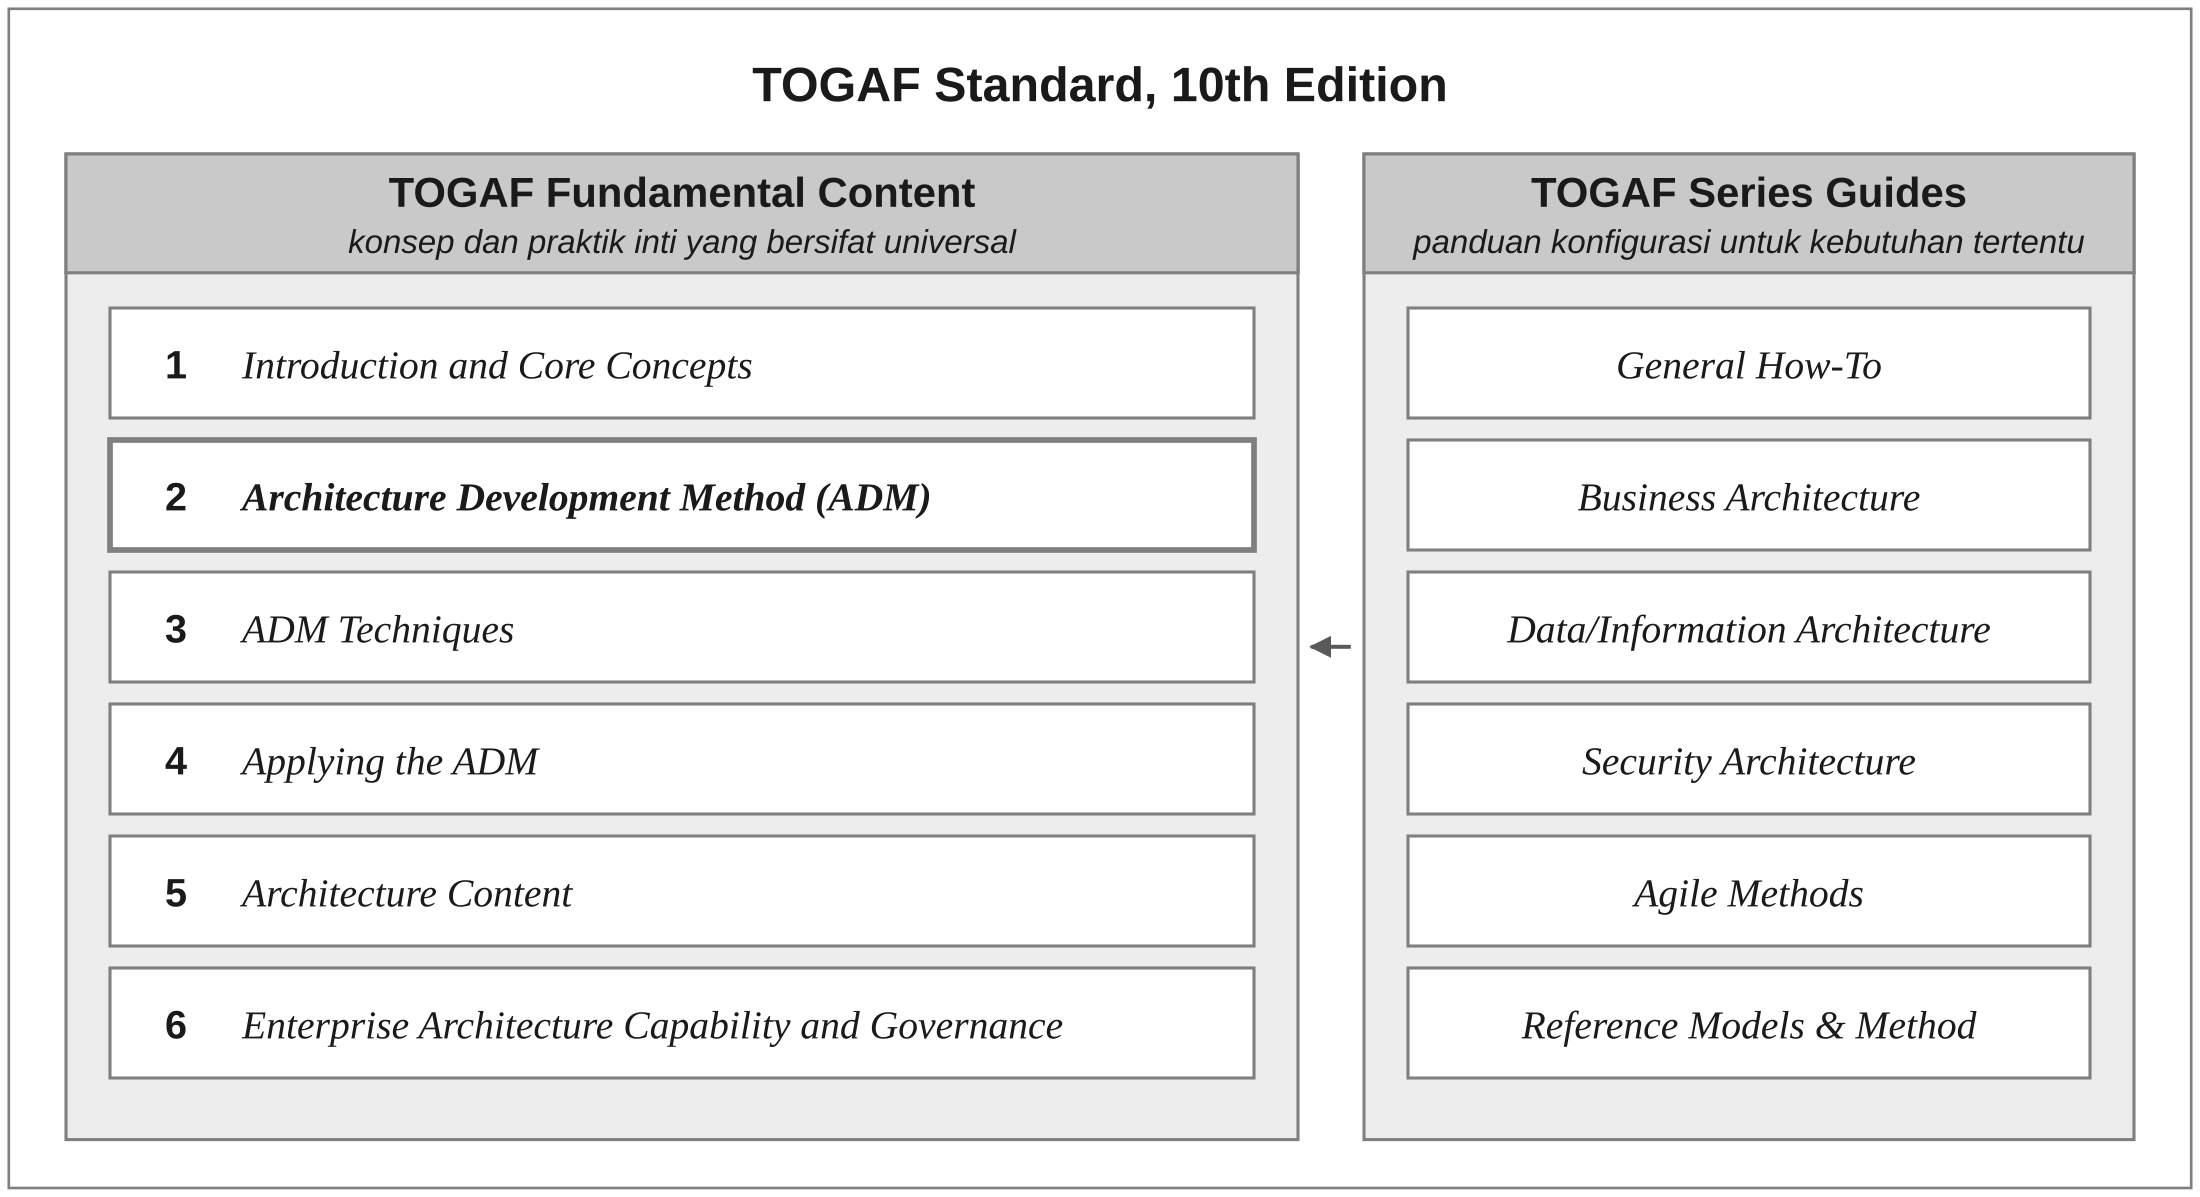
\includegraphics[width=1.00\linewidth,height=0.8\textheight,keepaspectratio]{images/Struktur TOGAF Standard 10th Edition.png}
\caption{Struktur \textit{TOGAF Standard, 10th Edition}}
\label{fig:II.9}
\end{figure}

Gambar~\ref{fig:II.9} menunjukkan bahwa \textit{TOGAF Fundamental Content} terdiri atas enam dokumen. \textit{Architecture Development Method} (ADM) merupakan inti TOGAF karena menyediakan proses yang teruji dan dapat diulang untuk mengembangkan arsitektur, sedangkan dokumen lainnya menopang ADM \cite{TOGAF2022}. Komponen TOGAF yang relevan bagi penelitian ini adalah ADM, \textit{Architecture Content Framework}, \textit{Enterprise Continuum}, dan \textit{Architecture Repository}, yang dibahas pada subbab berikut.

\subsection{Architecture Development Method}
\label{sec:II.4.2}

ADM merupakan metode untuk mengembangkan dan mengelola siklus hidup EA. ADM terdiri atas Fase \textit{Preliminary}, delapan fase pengembangan arsitektur, yaitu Fase A hingga Fase H, serta \textit{Requirements Management} yang berada di pusat siklus \cite{TOGAF2022}, sebagaimana ditunjukkan pada Gambar~\ref{fig:II.10}.

\begin{figure}[htbp]
\centering
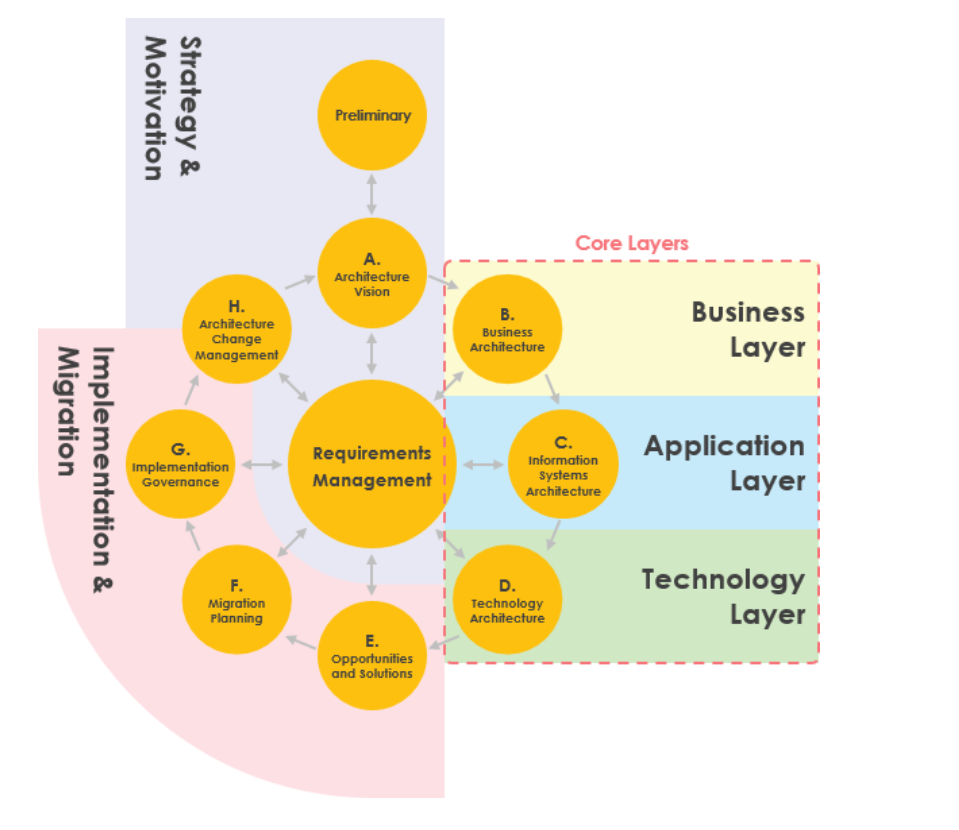
\includegraphics[width=0.79\linewidth,height=0.8\textheight,keepaspectratio]{images/Siklus TOGAF ADM.png}
\caption{Siklus TOGAF ADM}
\label{fig:II.10}
\end{figure}

Gambar~\ref{fig:II.10} menunjukkan bahwa Fase \textit{Preliminary} menjadi titik masuk siklus, kemudian Fase A hingga Fase H dijalankan secara berurutan. \textit{Requirements Management} berlangsung terus-menerus untuk memastikan setiap perubahan kebutuhan diteruskan ke seluruh fase \cite{TOGAF2022}. Gambar tersebut juga mengelompokkan fase ADM berdasarkan lapisan bahasa pemodelan ArchiMate \cite{ArchiMate2019}, yaitu \textit{Strategy \& Motivation} (Fase \textit{Preliminary}, Fase A, dan \textit{Requirements Management}), \textit{Core Layers} (Fase B, C, dan D), serta \textit{Implementation \& Migration} (Fase E hingga H). Tujuan setiap fase ADM disajikan pada Tabel~\ref{tab:II.3}.

\begingroup\small\setstretch{1.0}
\begin{longtable}{@{}>{\raggedright\arraybackslash\hspace{0pt}}p{0.318\linewidth}>{\raggedright\arraybackslash\hspace{0pt}}p{0.651\linewidth}@{}}
\caption{Fase TOGAF ADM dan Tujuannya}\label{tab:II.3}\\
\toprule
\textbf{Fase} & \textbf{Tujuan Utama}\\
\midrule
\endfirsthead
\multicolumn{2}{@{}l}{\small\itshape \tablename\ \thetable{} (lanjutan)}\\
\toprule
\textbf{Fase} & \textbf{Tujuan Utama}\\
\midrule
\endhead
\bottomrule
\endlastfoot
\textit{Preliminary} & Menetapkan kapabilitas arsitektur, termasuk prinsip arsitektur, tata kelola, dan penyesuaian \textit{framework}.\\*
A. \textit{Architecture Vision} & Menetapkan ruang lingkup, pemangku kepentingan, dan visi arsitektur, serta memperoleh persetujuan melalui \textit{Statement of Architecture Work}.\\
B. \textit{Business Architecture} & Mengembangkan arsitektur bisnis \textit{baseline} dan \textit{target} serta menganalisis kesenjangannya.\\
C. \textit{Information Systems Architectures} & Mengembangkan arsitektur data dan aplikasi \textit{baseline} dan \textit{target} serta menganalisis kesenjangannya.\\
D. \textit{Technology Architecture} & Mengembangkan arsitektur teknologi \textit{baseline} dan \textit{target} serta menganalisis kesenjangannya.\\
E. \textit{Opportunities and Solutions} & Mengidentifikasi paket pekerjaan dan arsitektur transisi untuk mewujudkan arsitektur \textit{target}.\\
F. \textit{Migration Planning} & Menyusun rencana implementasi dan migrasi beserta prioritasnya.\\
G. \textit{Implementation Governance} & Mengawasi implementasi agar sesuai dengan arsitektur \textit{target}.\\
H. \textit{Architecture Change Management} & Mengelola perubahan arsitektur secara berkelanjutan setelah implementasi.\\*
\textit{Requirements Management} & Mengelola kebutuhan arsitektur sepanjang siklus ADM.\\
\end{longtable}
\endgroup

Tabel~\ref{tab:II.3} menunjukkan bahwa setiap fase memiliki tujuan yang berbeda, tetapi saling terhubung dalam satu siklus. ADM juga bersifat generik, sehingga perlu disesuaikan (\textit{tailoring}) sejak Fase \textit{Preliminary} melalui penyesuaian terminologi, proses, dan konten agar sesuai dengan kebutuhan organisasi dan dapat diintegrasikan dengan \textit{framework} lain \cite{TOGAF2022}. Dalam penelitian ini, struktur fase ADM dipertahankan, sedangkan penyesuaian dilakukan pada masukan, langkah, dan keluaran fase yang memanfaatkan arsitektur referensi.

\subsection{Architecture Content Framework dan Content Metamodel}
\label{sec:II.4.3}

ADM menjelaskan cara mengembangkan arsitektur, sedangkan \textit{Architecture Content Framework} menjelaskan bentuk arsitektur yang dihasilkan \cite{TOGAF2022}. \textit{Content framework} mengelompokkan hasil kerja arsitektur ke dalam tiga kategori, yaitu sebagai berikut \cite{TOGAF2022}.

\begin{enumerate}[label=\arabic*.]
\item \textit{Deliverable}, yaitu produk kerja formal yang disepakati pemangku kepentingan, misalnya \textit{Architecture Definition Document}.
\item Artefak (\textit{artifact}), yaitu tampilan isi arsitektur, misalnya katalog, matriks, atau diagram alur proses.
\item \textit{Building block}, yaitu komponen arsitektur yang digambarkan oleh artefak, misalnya proses bisnis, aktor, aplikasi, atau layanan teknologi.
\end{enumerate}

\textit{Building block} dibedakan menjadi \textit{Architecture Building Block} (ABB\label{sk:ABB}) dan \textit{Solution Building Block} (SBB\label{sk:SBB}). ABB berkaitan dengan \textit{Architecture Continuum} serta ditetapkan atau dipilih melalui ADM, sedangkan SBB berkaitan dengan \textit{Solutions Continuum}, dapat dibeli atau dibangun, dan diperoleh dengan memperinci ABB secara bertahap. \textit{Building block} yang baik memiliki batas dan spesifikasi yang tidak terikat pada satu bentuk implementasi serta antarmuka yang stabil, sehingga mendukung interoperabilitas \cite{TOGAF2022}.

Hubungan antarelemen arsitektur diatur melalui \textit{enterprise metamodel}, yaitu model yang mendefinisikan jenis entitas dalam model \textit{enterprise} beserta hubungan antarentitas tersebut, misalnya entitas peran (\textit{role}), proses, aplikasi, dan layanan teknologi. TOGAF menganjurkan setiap organisasi menyusun \textit{metamodel} sesuai kebutuhannya \cite{TOGAF2022}. Konsep \textit{building block} dan \textit{metamodel} tersebut menjadi dasar perumusan komponen dan hubungan antarkomponen arsitektur referensi pada Bab III.

\subsection{Enterprise Continuum dan Architecture Repository}
\label{sec:II.4.4}

\textit{Enterprise Continuum} adalah cara mengklasifikasikan aset arsitektur dan solusi, mulai dari yang bersifat generik hingga yang spesifik bagi suatu organisasi. \textit{Enterprise Continuum} terdiri atas \textit{Architecture Continuum} dan \textit{Solutions Continuum} \cite{TOGAF2022}, sebagaimana ditunjukkan pada Gambar~\ref{fig:II.11}.

\begin{figure}[htbp]
\centering
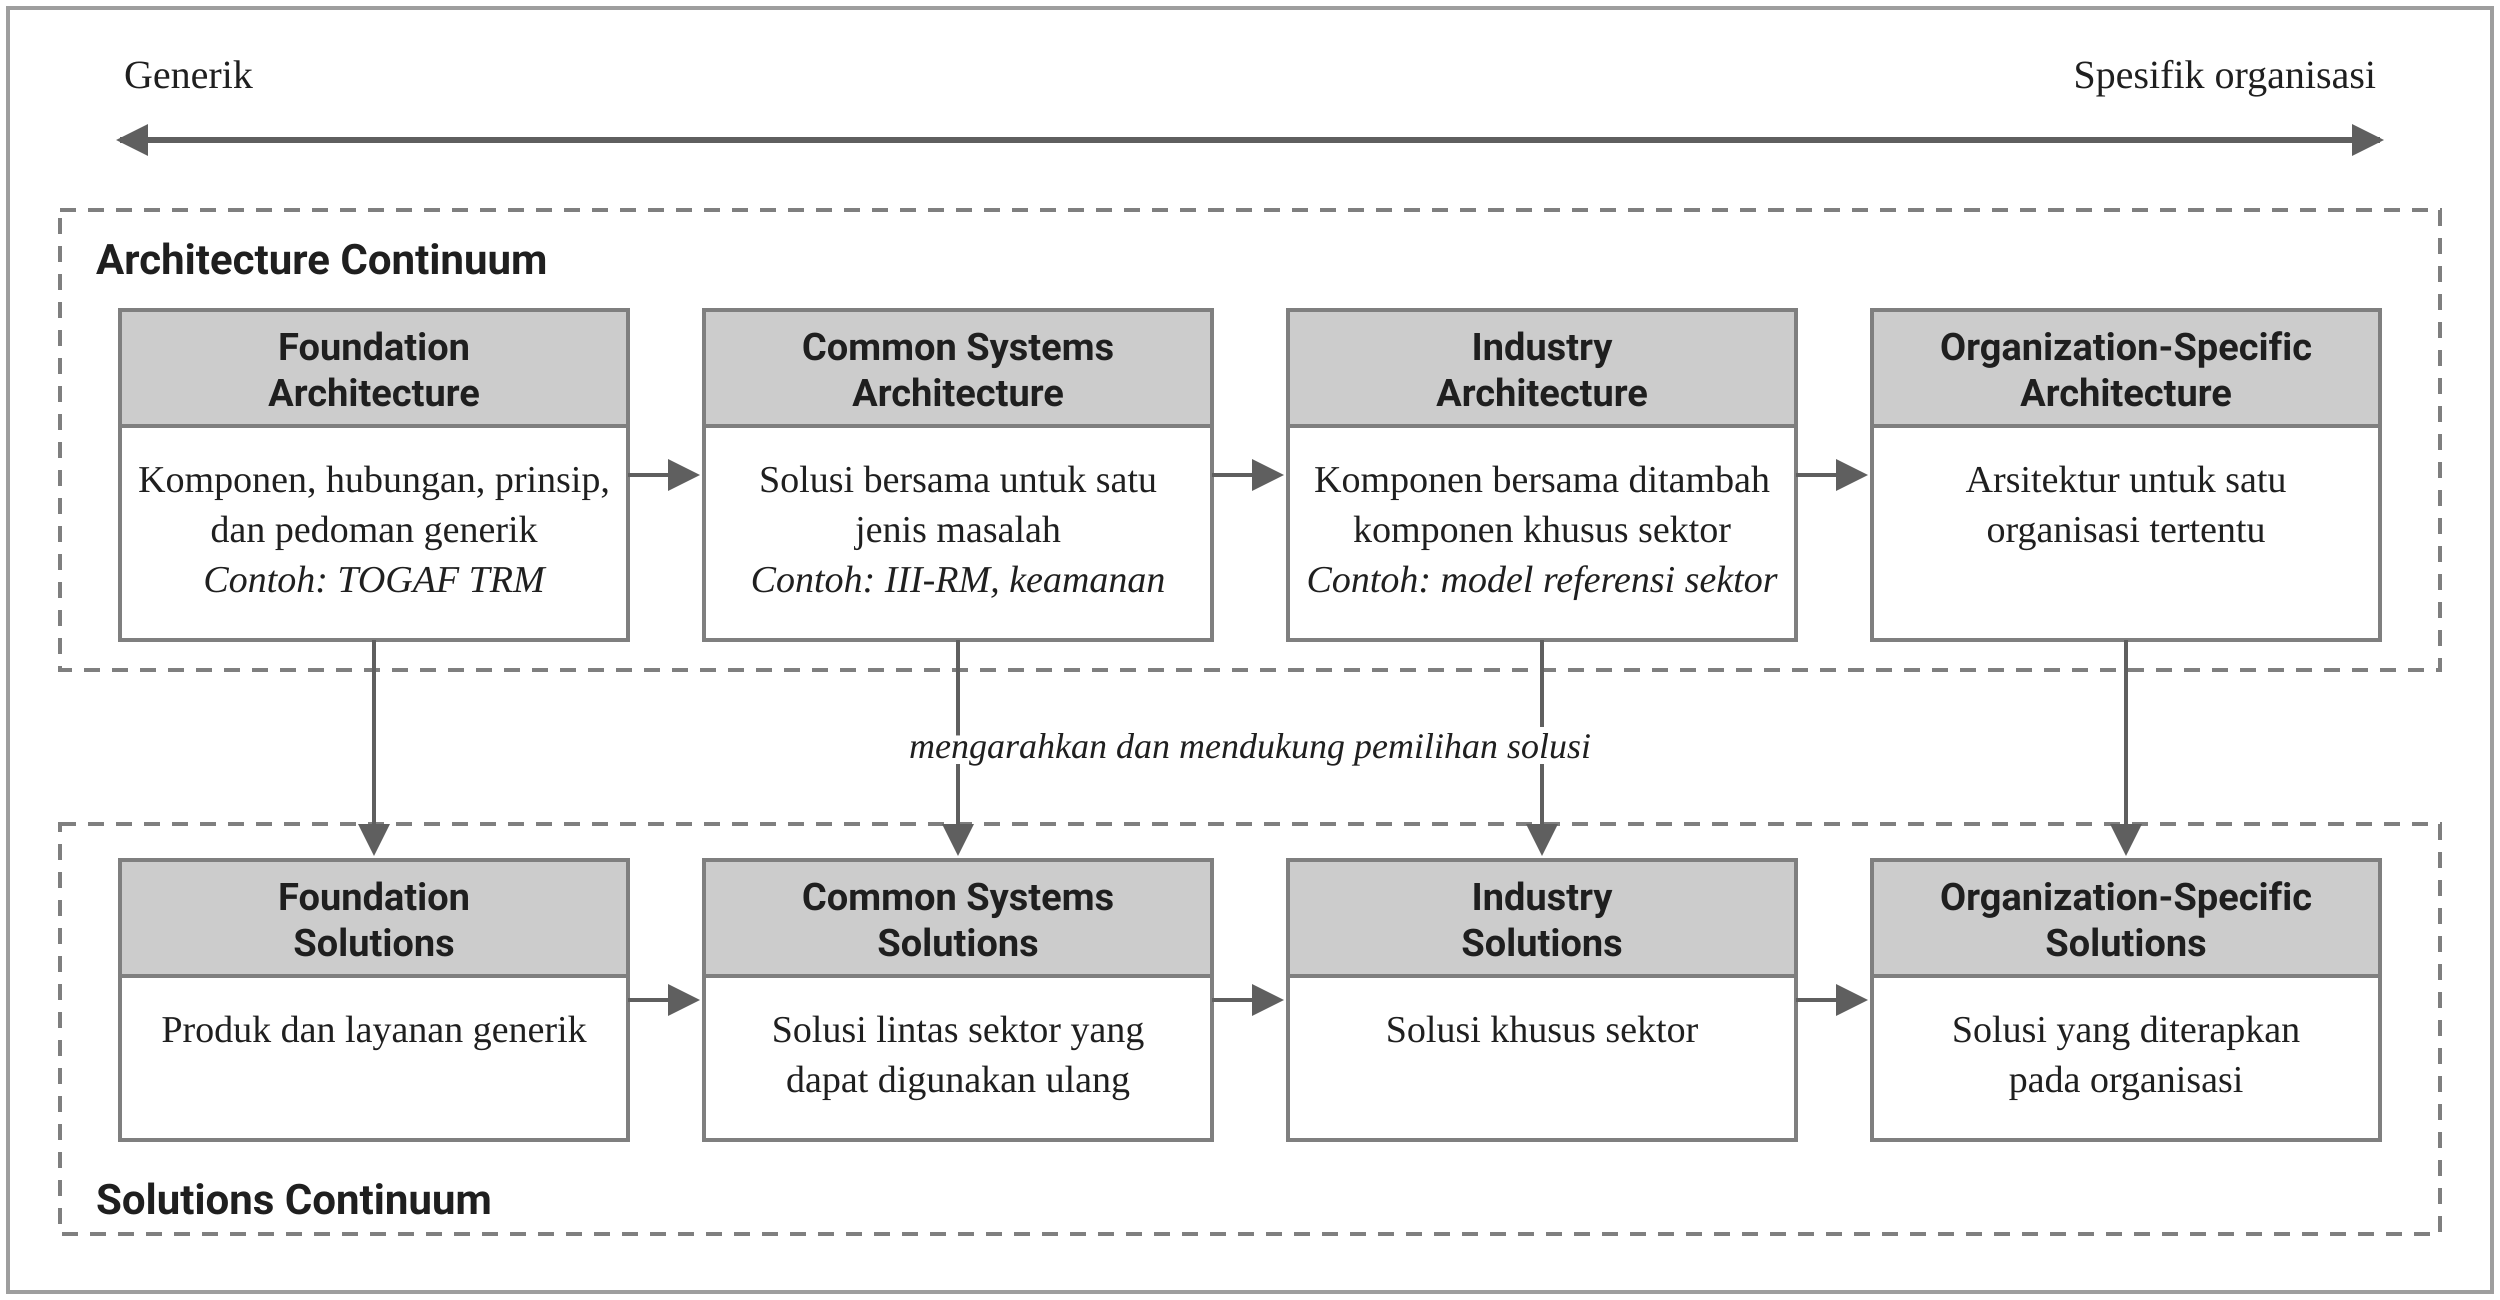
\includegraphics[width=1.00\linewidth,height=0.8\textheight,keepaspectratio]{images/Enterprise Continuum.png}
\caption{\textit{Enterprise Continuum}}
\label{fig:II.11}
\end{figure}

Gambar~\ref{fig:II.11} menunjukkan bahwa \textit{Architecture Continuum} terdiri atas empat tingkat. \textit{Foundation Architecture} memuat komponen, hubungan, prinsip, dan pedoman generik, misalnya TOGAF \textit{Technical Reference Model} (TRM\label{sk:TRM}). \textit{Common Systems Architecture} memuat solusi bersama untuk satu jenis masalah, seperti keamanan atau jaringan. \textit{Industry Architecture} memadukan komponen bersama dengan komponen khusus suatu sektor. \textit{Organization-Specific Architecture} mengarahkan penerapan solusi pada satu organisasi tertentu. Setiap tingkat arsitektur mengarahkan pemilihan solusi pada tingkat yang sama di \textit{Solutions Continuum}. Model referensi generik ditempatkan pada tingkat \textit{Foundation}, sedangkan model referensi suatu sektor ditempatkan pada tingkat \textit{Industry} \cite{TOGAF2022}.

\textit{Enterprise Continuum} didukung oleh \textit{Architecture Repository}, yaitu tempat penyimpanan keluaran arsitektur pada berbagai tingkat abstraksi \cite{TOGAF2022}. Kelas informasi dalam \textit{Architecture Repository} disajikan pada Tabel~\ref{tab:II.4}.

\begingroup\small\setstretch{1.0}
\begin{longtable}{@{}>{\raggedright\arraybackslash\hspace{0pt}}p{0.354\linewidth}>{\raggedright\arraybackslash\hspace{0pt}}p{0.615\linewidth}@{}}
\caption{Kelas Informasi dalam \textit{Architecture Repository}}\label{tab:II.4}\\
\toprule
\textbf{Kelas} & \textbf{Isi}\\
\midrule
\endfirsthead
\multicolumn{2}{@{}l}{\small\itshape \tablename\ \thetable{} (lanjutan)}\\
\toprule
\textbf{Kelas} & \textbf{Isi}\\
\midrule
\endhead
\bottomrule
\endlastfoot
\textit{Architecture Metamodel} & Versi \textit{framework} arsitektur yang telah disesuaikan, termasuk metode dan \textit{metamodel}-nya.\\*
\textit{Architecture Capability} & Parameter, struktur, dan proses yang mengatur repositori.\\
\textit{Architecture Landscape} & Aset arsitektur yang digunakan atau direncanakan pada waktu tertentu.\\
\textit{Standards Library} & Standar yang wajib dipenuhi oleh arsitektur baru.\\
\textit{Reference Library} & Arsitektur referensi, model referensi, pustaka \textit{viewpoint}, dan templat untuk mempercepat penyusunan arsitektur.\\
\textit{Governance Repository} & Catatan kegiatan tata kelola arsitektur.\\
\textit{Architecture Requirements Repository} & Kebutuhan arsitektur yang telah disetujui \textit{Architecture Board}.\\*
\textit{Solutions Landscape} & \textit{Solution building block} yang direncanakan atau telah diterapkan.\\
\end{longtable}
\endgroup

Tabel~\ref{tab:II.4} menunjukkan bahwa arsitektur referensi disimpan pada \textit{Reference Library}, yang dapat diklasifikasikan menggunakan \textit{Architecture Continuum} \cite{TOGAF2022}. Dengan demikian, TOGAF telah menyediakan tempat bagi arsitektur referensi sektoral, yaitu pada tingkat \textit{Industry Architecture} dan \textit{Reference Library}. Namun, TOGAF tidak menyediakan isi arsitektur referensi untuk sektor pertahanan, sehingga isi tersebut perlu dirancang.

\section{Framework EA Pertahanan}
\label{sec:II.5}

\textit{Framework} EA menyediakan struktur, sudut pandang (\textit{viewpoint}), dan panduan untuk mendeskripsikan serta mengembangkan arsitektur. Di lingkungan pertahanan, \textit{framework} EA yang banyak digunakan adalah DoDAF, NAF, dan MODAF \cite{Weilkiens2022}. Ketiganya berakar pada \textit{C4ISR Architecture Framework}, yaitu kerangka yang dikembangkan Departemen Pertahanan Amerika Serikat untuk menyeragamkan deskripsi arsitektur sistem komando, kendali, komunikasi, komputer, intelijen, pengawasan, dan pengintaian \cite{C4ISRAWG1998}. Perkembangan ketiga \textit{framework} tersebut ditunjukkan pada Gambar~\ref{fig:II.12}.

\begin{figure}[htbp]
\centering
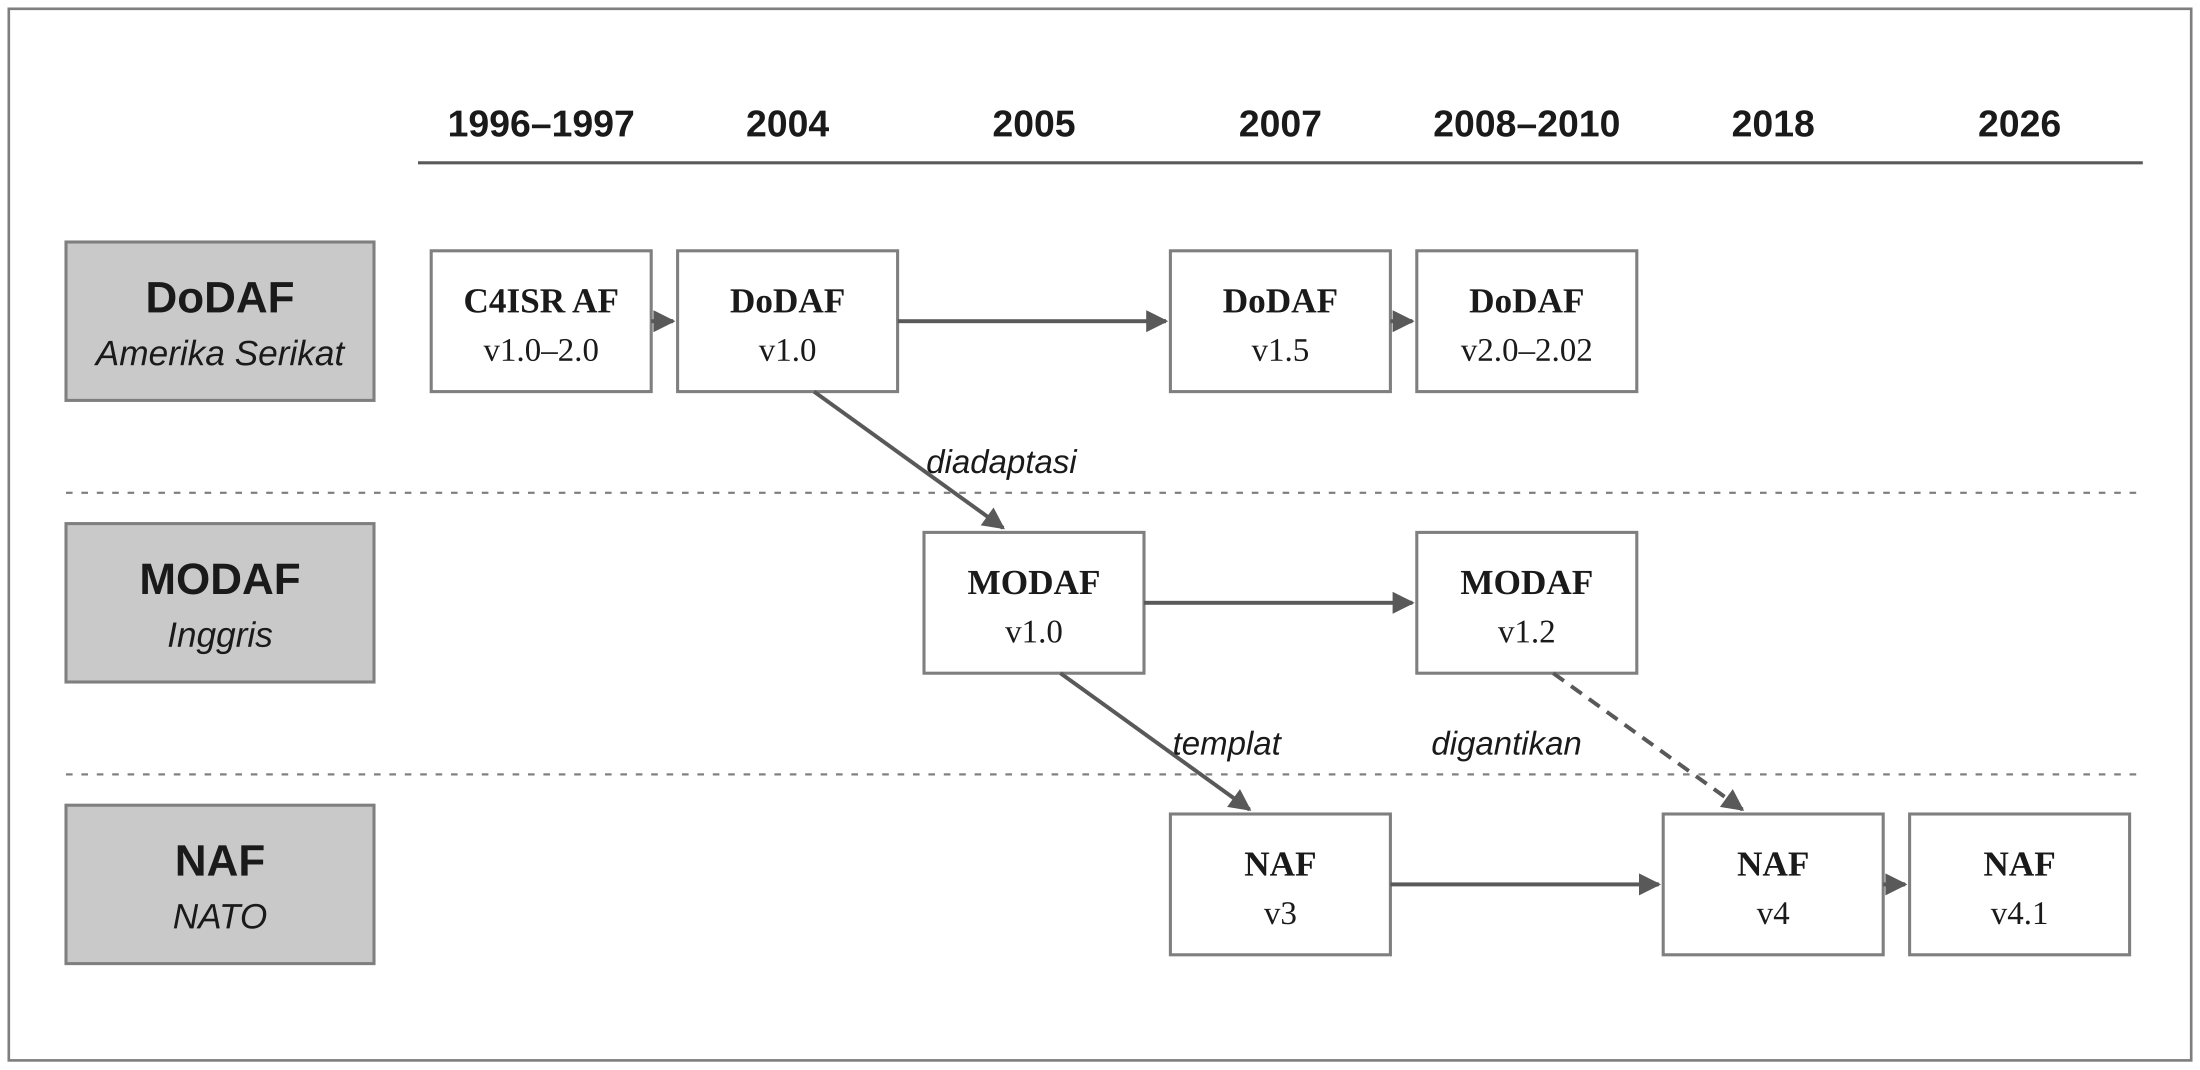
\includegraphics[width=1.00\linewidth,height=0.8\textheight,keepaspectratio]{images/Perkembangan Framework EA Pertahanan.png}
\caption{Perkembangan \textit{Framework} EA Pertahanan}
\label{fig:II.12}
\end{figure}

Gambar~\ref{fig:II.12} menunjukkan bahwa DoDAF berkembang langsung dari \textit{C4ISR Architecture Framework}. MODAF diadaptasi dari DoDAF versi 1.0 dan menjadi acuan bagi NAF versi 3, kemudian digantikan oleh NAF versi 4 \cite{MODAF2012}. Karena memiliki akar yang sama, ketiga \textit{framework} tersebut kuat dalam merepresentasikan kapabilitas, operasi, dan interoperabilitas sistem militer.

\subsection{DoDAF}
\label{sec:II.5.1}

\textit{Department of Defense Architecture Framework} (DoDAF) dikembangkan Departemen Pertahanan Amerika Serikat untuk mendukung pengambilan keputusan melalui pengorganisasian dan berbagi informasi lintas departemen, komponen, dan program. Perubahan terpenting terjadi pada versi 2.0, yaitu pergeseran dari pendekatan berbasis produk menjadi berbasis data melalui \textit{DoDAF Meta Model} (DM2\label{sk:DM2}), sehingga model arsitektur dapat dipilih sesuai tujuan penggunaannya (\textit{fit-for-purpose}). DoDAF 2.02 mengelompokkan 52 model ke dalam delapan \textit{viewpoint} \cite{DoDAF2010v202}, sebagaimana ditunjukkan pada Gambar~\ref{fig:II.13}.

\begin{figure}[htbp]
\centering
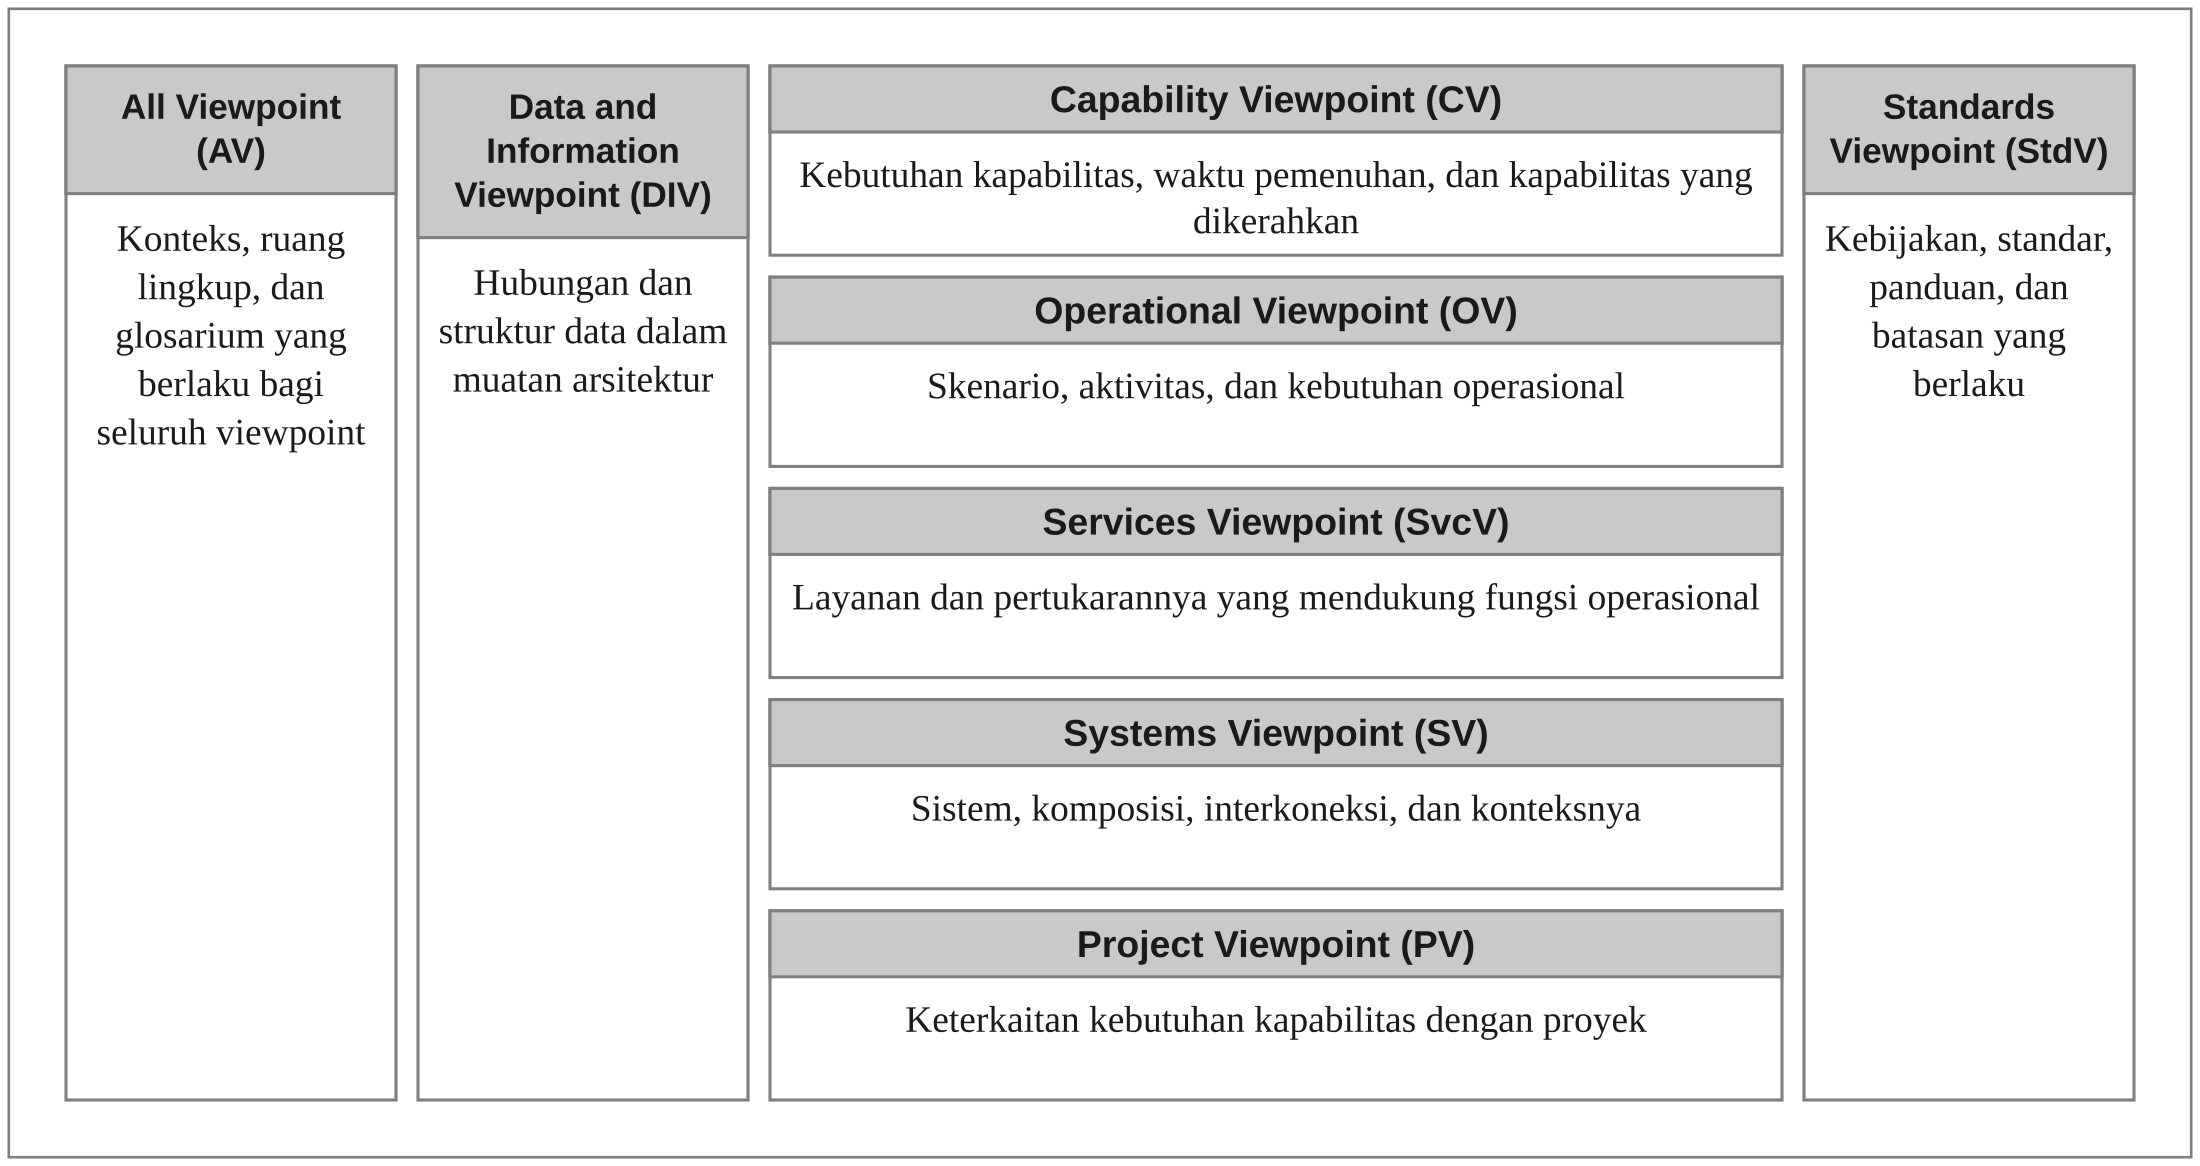
\includegraphics[width=1.00\linewidth,height=0.8\textheight,keepaspectratio]{images/Viewpoint DoDAF 202.png}
\caption{\textit{Viewpoint} DoDAF 2.02}
\label{fig:II.13}
\end{figure}

Gambar~\ref{fig:II.13} menunjukkan bahwa \textit{All Viewpoint}, \textit{Data and Information Viewpoint}, dan \textit{Standards Viewpoint} berlaku bagi seluruh model, sedangkan \textit{Capability}, \textit{Operational}, \textit{Services}, \textit{Systems}, dan \textit{Project Viewpoint} menggambarkan arsitektur mulai dari kebutuhan kapabilitas hingga implementasinya. DoDAF menyediakan enam langkah pengembangan yang bersifat umum, sedangkan sebagian besar muatannya berupa ketentuan tentang apa yang harus dideskripsikan untuk mendukung proses inti Departemen Pertahanan Amerika Serikat, seperti pengembangan kapabilitas, penganggaran, dan akuisisi \cite{DoDAF2010v202}.

\subsection{NAF}
\label{sec:II.5.2}

\textit{NATO Architecture Framework} (NAF) dikembangkan NATO sebagai standar untuk mengembangkan dan mendeskripsikan arsitektur militer maupun bisnis. Versi terbarunya, NAFv4.1, diterbitkan pada Maret 2026 oleh \textit{Architecture Capability Team} di bawah \textit{Digital Policy Committee}. NAFv4 terdiri atas metodologi pengembangan arsitektur, \textit{viewpoint}, dan meta-model yang memanfaatkan meta-model komersial seperti ArchiMate dan UAF\label{sk:UAF} \cite{NAFv41}. \textit{Viewpoint} NAFv4 disusun dalam \textit{grid} dua dimensi, yaitu subjek perhatian sebagai baris dan aspek perhatian sebagai kolom \cite{NAFv41,Lundberg2026}, sebagaimana ditunjukkan pada Gambar~\ref{fig:II.14}.

\begin{figure}[htbp]
\centering
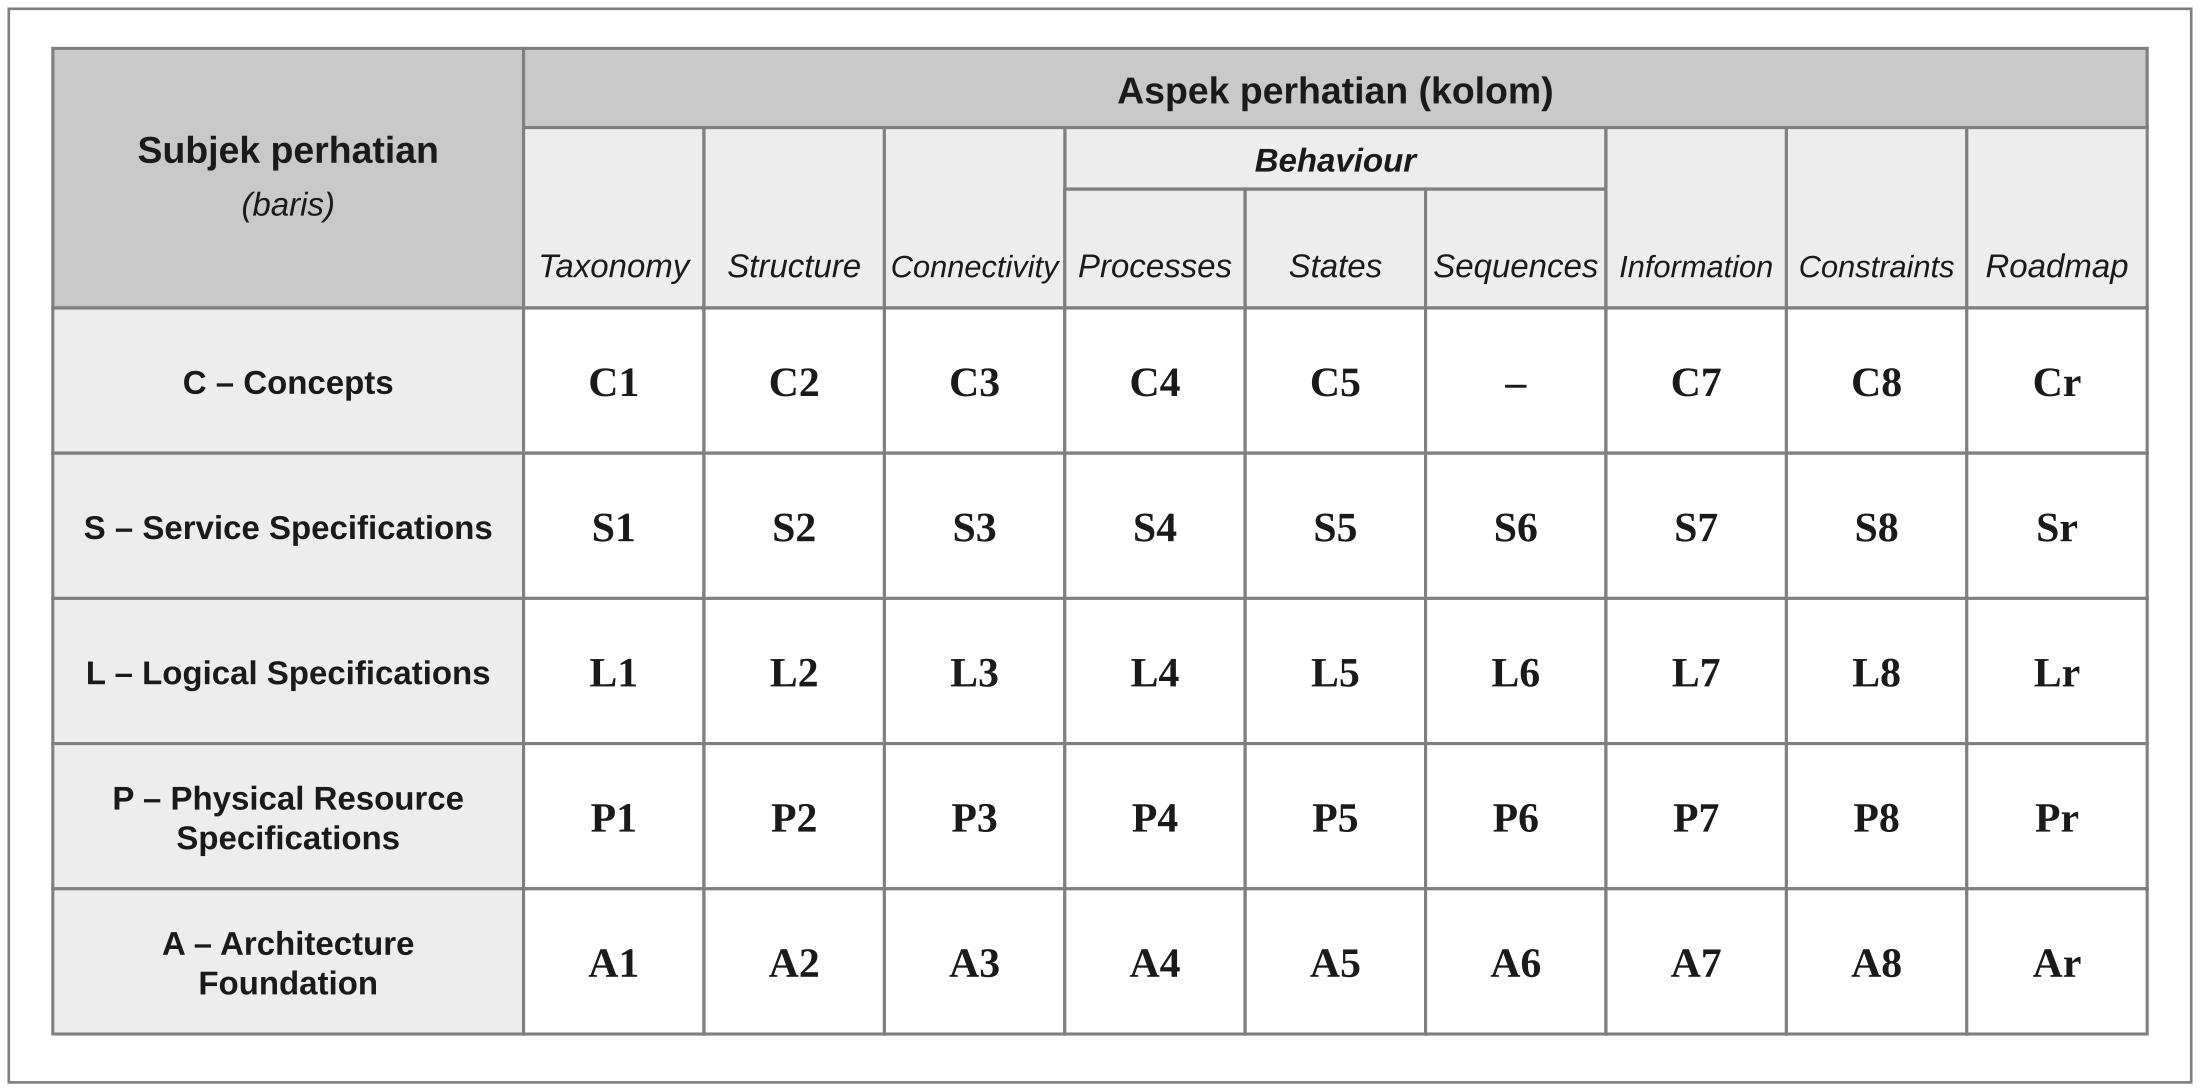
\includegraphics[width=1.00\linewidth,height=0.8\textheight,keepaspectratio]{images/Grid Viewpoint NAFv41.png}
\caption{\textit{Grid Viewpoint} NAFv4.1}
\label{fig:II.14}
\end{figure}

Gambar~\ref{fig:II.14} menunjukkan bahwa setiap sel \textit{grid} merupakan satu \textit{viewpoint}, misalnya C1 \textit{Capability Taxonomy} dan Cr \textit{Capability Roadmap}. Berbeda dengan DoDAF, NAFv4 dilengkapi metodologi delapan tahap, mulai dari penetapan \textit{architecture landscape} hingga pengelolaan perubahan arsitektur \cite{NAFv41}. Namun, NAF dirancang untuk interoperabilitas multinasional dan mengikuti kebijakan NATO, sehingga penerapannya di Indonesia memerlukan penyesuaian terhadap kebijakan nasional.

\subsection{MODAF}
\label{sec:II.5.3}

\textit{Ministry of Defence Architecture Framework} (MODAF) dikembangkan Kementerian Pertahanan Inggris untuk mendukung perencanaan pertahanan dan manajemen perubahan. MODAF diadaptasi dari DoDAF versi 1.0 dan menambahkan \textit{Strategic Views} serta \textit{Acquisition Views} untuk mendukung pengelolaan kapabilitas dan program pengadaan \cite{Weilkiens2022,MODAF2012}. MODAF memiliki tujuh \textit{viewpoint} \cite{MODAF2012}, sebagaimana ditunjukkan pada Gambar~\ref{fig:II.15}.

\begin{figure}[htbp]
\centering
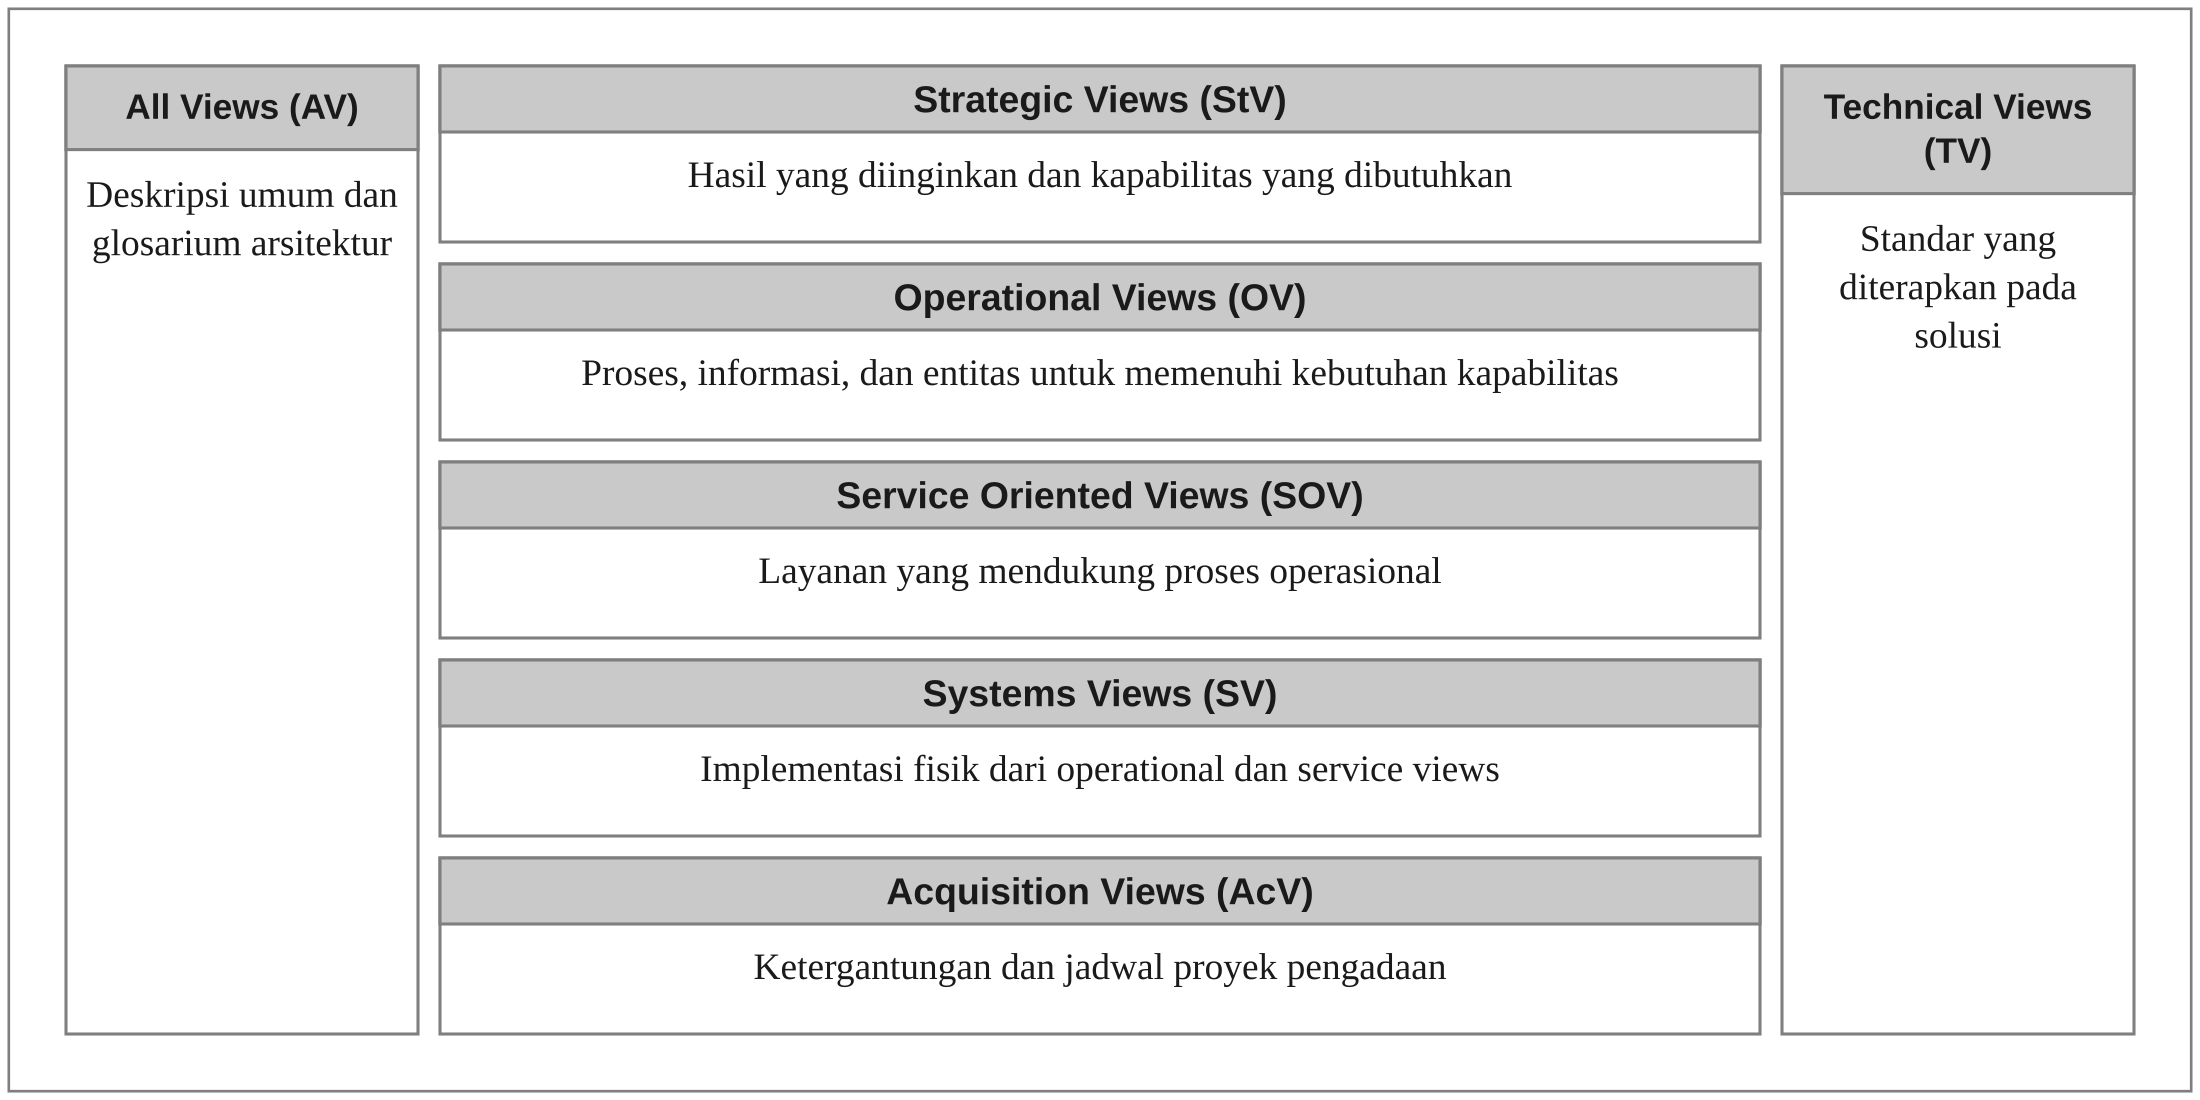
\includegraphics[width=1.00\linewidth,height=0.8\textheight,keepaspectratio]{images/Viewpoint MODAF.png}
\caption{\textit{Viewpoint} MODAF}
\label{fig:II.15}
\end{figure}

Gambar~\ref{fig:II.15} menunjukkan bahwa \textit{Strategic Views} menetapkan kapabilitas yang dibutuhkan, kemudian kapabilitas tersebut dijabarkan ke dalam \textit{Operational}, \textit{Service Oriented}, dan \textit{Systems Views}, sedangkan \textit{Acquisition Views} menggambarkan ketergantungan dan jadwal proyek pengadaan. MODAF kini telah digantikan oleh NAFv4 \cite{MODAF2012}, sehingga dalam penelitian ini MODAF menjadi rujukan konsep \textit{viewpoint} strategis dan akuisisi.

\subsection{UAF}
\label{sec:II.5.4}

\textit{Unified Architecture Framework} (UAF) merupakan standar \textit{Object Management Group} (OMG\label{sk:OMG}) untuk menyusun deskripsi arsitektur bagi industri, instansi pemerintah, dan organisasi pertahanan. UAF dikembangkan dari \textit{Unified Profile for DoDAF and MODAF} (UPDM\label{sk:UPDM}) dengan kebutuhan yang diturunkan dari DoDAF, MODAF, dan NAF, sehingga dapat menghasilkan produk arsitektur ketiga \textit{framework} tersebut \cite{OMGUAF2022}.

UAF versi 1.2 terdiri atas dua bagian normatif, yaitu \textit{Domain Metamodel} (DMM\label{sk:DMM}) yang mendefinisikan konsep dan hubungan antarkonsep, serta \textit{UAF Modeling Language} (UAFML\label{sk:UAFML}) yang mengimplementasikan DMM menggunakan UML\label{sk:UML} dan SysML\label{sk:SysML}. Kedua bagian tersebut juga diadopsi sebagai standar ISO\label{sk:ISO}/IEC\label{sk:IEC} 19540:2022 \cite{OMGUAF2022}. Dengan demikian, UAF berperan sebagai bahasa pemodelan dan meta-model bersama bagi \textit{framework} pertahanan, bukan sebagai metode pengembangan arsitektur maupun muatan acuan bagi organisasi tertentu.

\subsection{Perbandingan Framework EA}
\label{sec:II.5.5}

Perbandingan DoDAF, NAF, MODAF, UAF, dan TOGAF ditunjukkan pada Tabel~\ref{tab:II.5}.

\begingroup\small\setstretch{1.0}
\begin{longtable}{@{}>{\raggedright\arraybackslash\hspace{0pt}}p{0.137\linewidth}>{\raggedright\arraybackslash\hspace{0pt}}p{0.142\linewidth}>{\raggedright\arraybackslash\hspace{0pt}}p{0.142\linewidth}>{\raggedright\arraybackslash\hspace{0pt}}p{0.142\linewidth}>{\raggedright\arraybackslash\hspace{0pt}}p{0.142\linewidth}>{\raggedright\arraybackslash\hspace{0pt}}p{0.142\linewidth}@{}}
\caption{Perbandingan \textit{Framework} EA}\label{tab:II.5}\\
\toprule
\textbf{Aspek} & \textbf{DoDAF} & \textbf{NAF} & \textbf{MODAF} & \textbf{UAF} & \textbf{TOGAF}\\
\midrule
\endfirsthead
\multicolumn{6}{@{}l}{\small\itshape \tablename\ \thetable{} (lanjutan)}\\
\toprule
\textbf{Aspek} & \textbf{DoDAF} & \textbf{NAF} & \textbf{MODAF} & \textbf{UAF} & \textbf{TOGAF}\\
\midrule
\endhead
\bottomrule
\endlastfoot
Pengembang & Departemen Pertahanan Amerika Serikat & NATO & Kementerian Pertahanan Inggris & OMG & The Open Group\\*
Versi dan status & 2.02 (2010), berlaku & 4.1 (2026), berlaku & 1.2.004 (2010), digantikan NAFv4 & 1.2 (2022), ISO/IEC 19540:2022 & \textit{10th Edition} (2022), berlaku\\
Orientasi utama & Proses inti DoD: kapabilitas, anggaran, akuisisi & Interoperabilitas NATO & Perencanaan pertahanan Inggris & Bahasa pemodelan dan meta-model arsitektur & EA generik lintas sektor\\
Struktur utama & 8 \textit{viewpoint}, 52 model, DM2 & \textit{Grid viewpoint}, meta-model ArchiMate dan UAF & 7 \textit{viewpoint}, meta-model M3 & DMM dan UAFML (UML/SysML) & \textit{Fundamental Content}, \textit{Series Guides}, 4 domain\\
Metode pengembangan & 6 langkah umum & 8 tahap & Tidak baku & Tidak menetapkan metode & ADM iteratif\\
Muatan pertahanan & Kuat & Kuat & Kuat & Kuat & Tidak tersedia\\*
Keselarasan dengan Arsitektur SPBE & Perlu pemetaan ulang & Perlu pemetaan ulang & Perlu pemetaan ulang & Perlu pemetaan ulang & Domain berpadanan (Tabel~\ref{tab:II.2})\\
\end{longtable}
\endgroup

Tabel~\ref{tab:II.5} menunjukkan bahwa DoDAF, NAF, dan MODAF kuat dalam muatan pertahanan, tetapi terutama menetapkan apa yang harus dideskripsikan dan terikat pada kebijakan negara atau aliansi pengembangnya. UAF menyediakan bahasa pemodelan bersama, tetapi tidak menyediakan metode pengembangan. Sebaliknya, TOGAF menyediakan metode yang lengkap melalui ADM, domainnya berpadanan dengan Arsitektur SPBE, serta menyediakan tempat bagi arsitektur referensi melalui \textit{Enterprise Continuum}, tetapi tidak memiliki muatan pertahanan \cite{TOGAF2022}.

Perbandingan tersebut juga menunjukkan bahwa tidak satu pun \textit{framework} menyediakan muatan acuan yang siap diturunkan menjadi arsitektur organisasi pertahanan Indonesia. \textit{Framework} menjelaskan cara mendeskripsikan dan mengembangkan arsitektur, sedangkan muatan acuan yang dapat digunakan ulang disediakan oleh arsitektur referensi. Oleh karena itu, penelitian ini menggunakan TOGAF ADM sebagai metode penerapan, memanfaatkan \textit{viewpoint} kapabilitas dan operasional dari \textit{framework} pertahanan sebagai rujukan, dan merancang muatan pertahanan dalam bentuk arsitektur referensi.

\section{Arsitektur Referensi}
\label{sec:II.6}

Subbab ini membahas konsep arsitektur referensi, perbedaannya dengan model referensi, komponennya, kedudukannya dalam TOGAF, metode pengembangan dan evaluasinya, serta CSPA\label{sk:CSPA} sebagai contoh arsitektur referensi sektoral.

\subsection{Konsep dan Karakteristik Arsitektur Referensi}
\label{sec:II.6.1}

Cloutier dkk. menyatakan bahwa arsitektur referensi menghimpun pengetahuan arsitektur yang terakumulasi dari banyak pengembangan, mulai dari alasan (\textit{why}), apa yang dibangun (\textit{what}), hingga cara membangunnya (\textit{how}), dengan tujuan memberikan panduan bagi pengembangan selanjutnya \cite{Cloutier2010}. Angelov dkk. mendefinisikan arsitektur referensi sebagai arsitektur generik untuk suatu kelas sistem informasi yang menjadi dasar perancangan arsitektur konkret dari kelas tersebut \cite{Angelov2009}. Di lingkungan pertahanan, Departemen Pertahanan Amerika Serikat memandang arsitektur referensi sebagai sumber otoritatif yang mengarahkan dan membatasi pengembangan berbagai arsitektur dan solusi \cite{DoDCIO2010RA}.

Dari definisi tersebut, arsitektur referensi memiliki empat karakteristik, yaitu sebagai berikut.

\begin{enumerate}[label=\arabic*.]
\item Generik, yaitu berlaku untuk satu kelas organisasi atau sistem, bukan untuk satu organisasi tertentu.
\item Dapat digunakan ulang, yaitu menjadi dasar bagi banyak arsitektur konkret.
\item Mengarahkan dan membatasi, yaitu menetapkan arah sekaligus batasan bagi arsitektur turunannya.
\item Berbasis pengetahuan yang teruji, yaitu disusun dari praktik, standar, dan pengalaman yang telah terbukti.
\end{enumerate}

Angelov dkk. juga menunjukkan bahwa efektivitas arsitektur referensi ditentukan oleh kesesuaian (\textit{congruence}) antara konteks, tujuan, dan desainnya \cite{Angelov2012}. Artinya, arsitektur referensi perlu dirancang sesuai dengan konteks penggunanya, termasuk regulasi dan kelembagaan di sektor tersebut.

\subsection{Model Referensi dan Arsitektur Referensi}
\label{sec:II.6.2}

Istilah model referensi dan arsitektur referensi sering digunakan secara bergantian, padahal keduanya berbeda tingkat abstraksinya. OASIS\label{sk:OASIS} mendefinisikan model referensi sebagai kerangka abstrak untuk memahami entitas penting dan hubungan antarentitas dalam suatu lingkungan, yang tidak terikat pada standar, teknologi, atau detail implementasi tertentu. Satu model referensi dapat menjadi dasar bagi satu atau lebih arsitektur referensi \cite{OASISSOARM2006}. Hubungan tersebut ditunjukkan pada Gambar~\ref{fig:II.16}.

\begin{figure}[htbp]
\centering
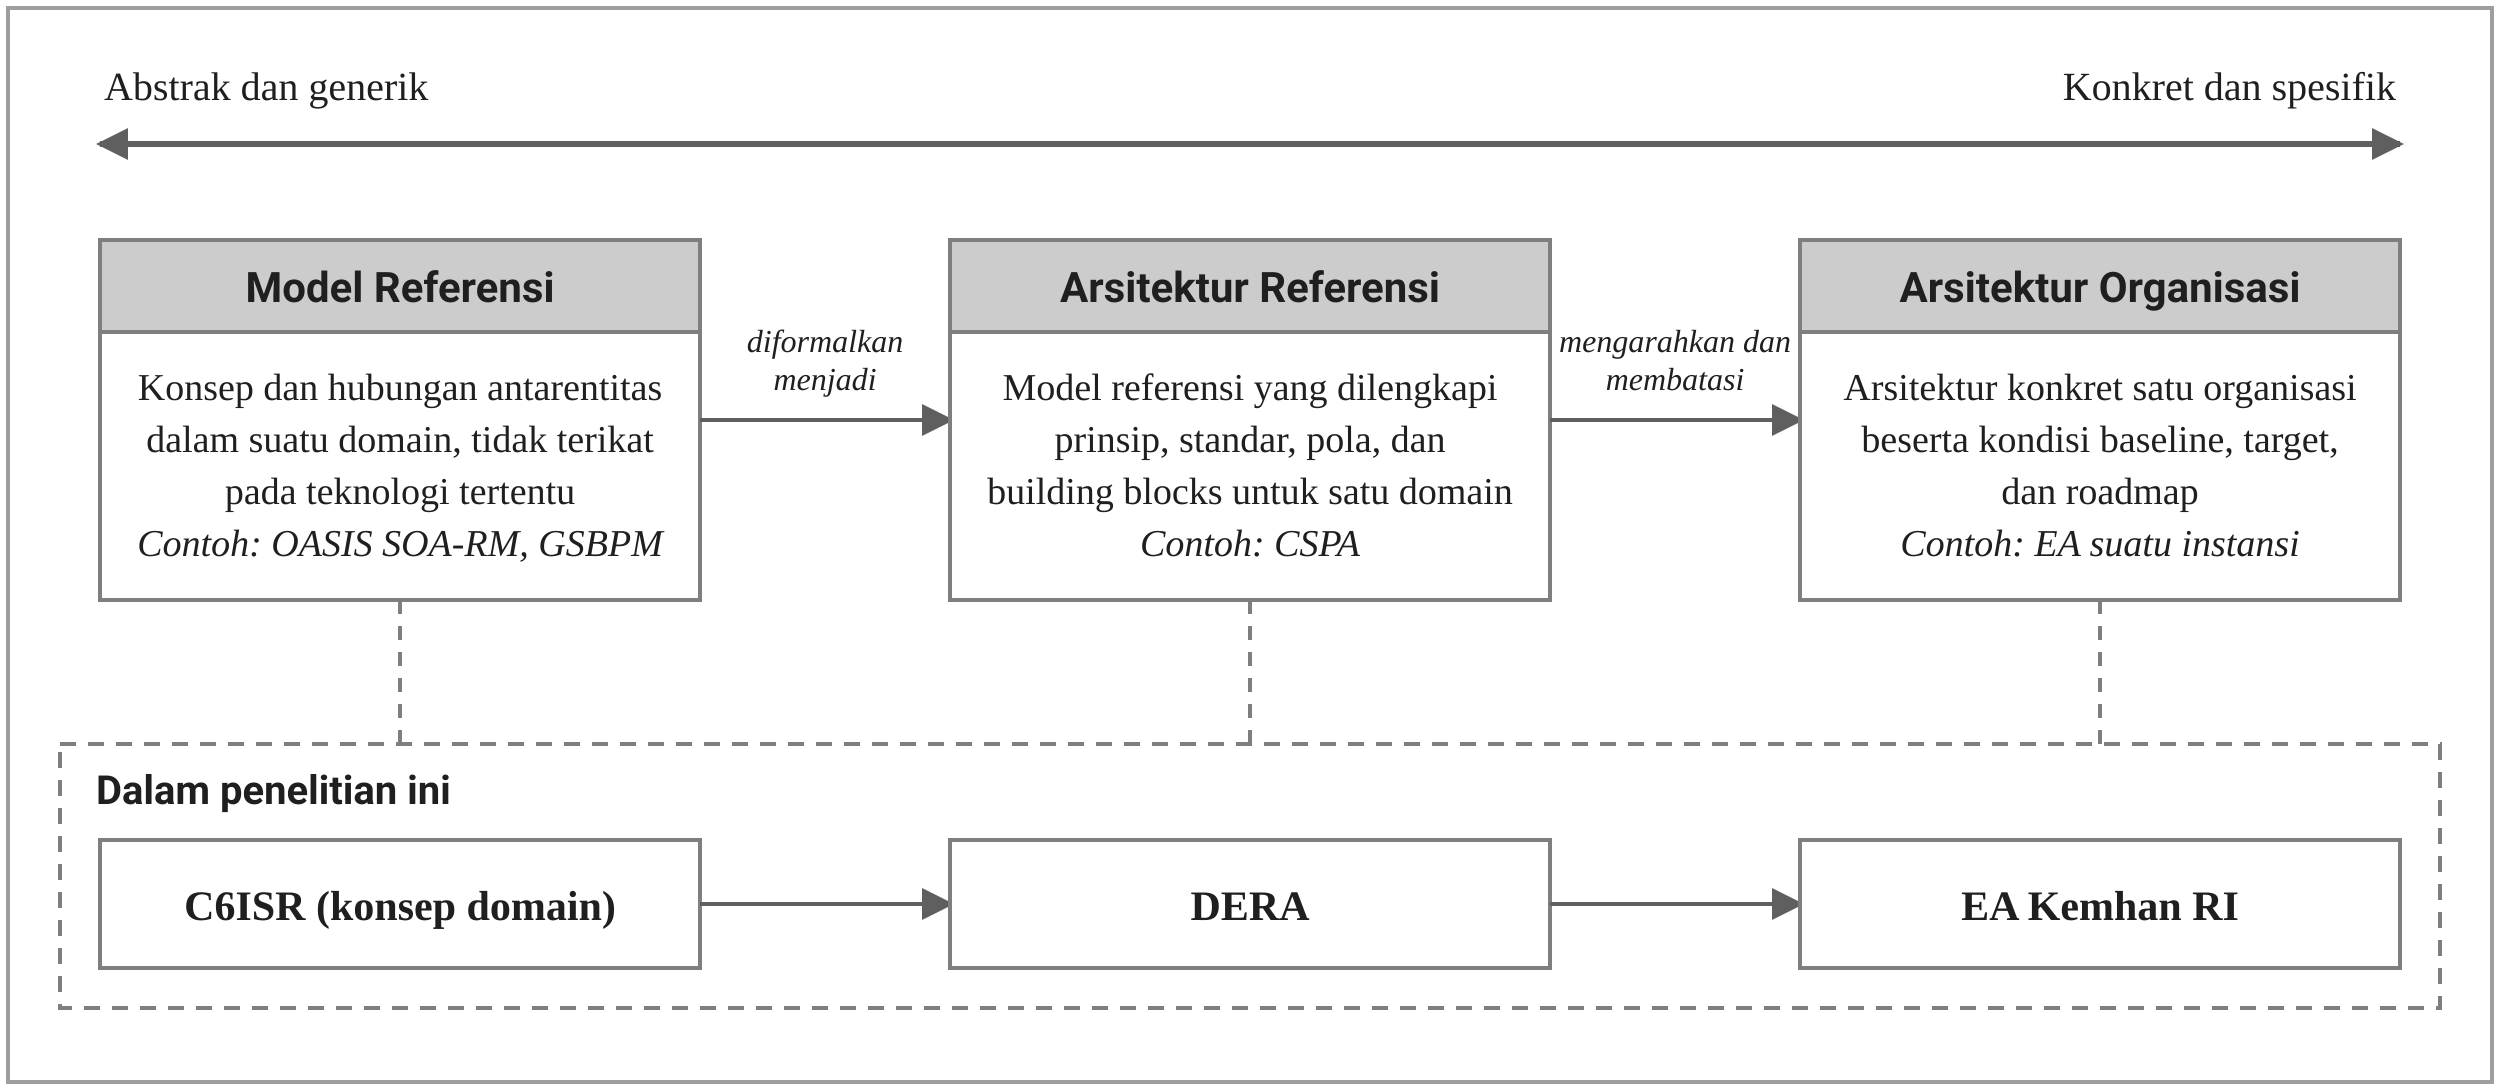
\includegraphics[width=1.00\linewidth,height=0.8\textheight,keepaspectratio]{images/Model Referensi Arsitektur Referensi dan Arsitektur Organisasi.png}
\caption{Model Referensi, Arsitektur Referensi, dan Arsitektur Organisasi}
\label{fig:II.16}
\end{figure}

Gambar~\ref{fig:II.16} menunjukkan bahwa model referensi hanya memuat konsep dan hubungannya. Arsitektur referensi melengkapi model referensi dengan prinsip, standar, pola, dan \textit{building blocks}, sehingga dapat mengarahkan dan membatasi arsitektur organisasi. Dalam penelitian ini, C6ISR berada pada tingkat model referensi karena baru berupa konsep domain. Penelitian ini merumuskan C6ISR menjadi arsitektur referensi, yaitu DERA, kemudian menurunkannya menjadi EA Kemhan RI.

\subsection{Komponen Arsitektur Referensi}
\label{sec:II.6.3}

Departemen Pertahanan Amerika Serikat menetapkan lima komponen arsitektur referensi \cite{DoDCIO2010RA}, sebagaimana disajikan pada Tabel~\ref{tab:II.6}.

\begingroup\small\setstretch{1.0}
\begin{longtable}{@{}>{\raggedright\arraybackslash\hspace{0pt}}p{0.257\linewidth}>{\raggedright\arraybackslash\hspace{0pt}}p{0.712\linewidth}@{}}
\caption{Komponen Arsitektur Referensi}\label{tab:II.6}\\
\toprule
\textbf{Komponen} & \textbf{Uraian}\\
\midrule
\endfirsthead
\multicolumn{2}{@{}l}{\small\itshape \tablename\ \thetable{} (lanjutan)}\\
\toprule
\textbf{Komponen} & \textbf{Uraian}\\
\midrule
\endhead
\bottomrule
\endlastfoot
Tujuan strategis (\textit{strategic purpose}) & Tujuan, ruang lingkup, dan permasalahan yang hendak diselesaikan oleh arsitektur referensi.\\*
Prinsip (\textit{principles}) & Pernyataan dasar tentang aturan, budaya, dan nilai yang mendorong posisi teknis dan pola.\\
Posisi teknis (\textit{technical positions}) & Panduan teknis dan standar yang harus diikuti dalam solusi.\\
Pola (\textit{patterns}) & Representasi arsitektur yang digeneralisasi untuk menunjukkan hubungan antarelemen.\\*
Kosakata (\textit{vocabulary}) & Istilah, akronim, dan definisi yang digunakan bersama oleh arsitektur turunannya.\\
\end{longtable}
\endgroup

Tabel~\ref{tab:II.6} menunjukkan bahwa arsitektur referensi tidak cukup berupa katalog atau gambar konseptual, tetapi juga harus memuat prinsip, posisi teknis, dan pola yang menghubungkan elemen-elemennya. Kelima komponen tersebut menjadi acuan struktur DERA pada Bab III.

\subsection{Arsitektur Referensi dalam TOGAF}
\label{sec:II.6.4}

Sebagaimana dibahas pada II.4.4, TOGAF menempatkan arsitektur referensi sektoral pada tingkat \textit{Industry Architecture} dalam \textit{Enterprise Continuum} dan menyimpannya dalam \textit{Reference Library} \cite{TOGAF2022}. Selain itu, ADM secara eksplisit memanfaatkan arsitektur dan model referensi. Fase \textit{Business Architecture}, \textit{Information Systems Architectures}, dan \textit{Technology Architecture} masing-masing diawali dengan langkah \textit{Select Reference Models, Viewpoints, and Tools}, dengan masukan dari \textit{Architecture Repository} berupa \textit{building blocks} yang dapat digunakan ulang, model referensi publik, model referensi khusus organisasi, dan standar organisasi \cite{TOGAF2022}.

Mekanisme tersebut menunjukkan bahwa arsitektur referensi dapat digunakan dalam ADM tanpa mengubah struktur fasenya. Arsitektur referensi berperan sebagai masukan pada langkah awal setiap fase arsitektur, sedangkan penyesuaian dilakukan pada masukan, langkah, dan keluaran fase yang relevan.

\subsection{Metode Pengembangan dan Evaluasi Arsitektur Referensi}
\label{sec:II.6.5}

Galster dan Avgeriou mengusulkan enam langkah untuk merancang arsitektur referensi yang berbasis bukti empiris \cite{Galster2011}, yaitu sebagai berikut.

\begin{enumerate}[label=\arabic*.]
\item Menentukan jenis arsitektur referensi.
\item Memilih strategi perancangan.
\item Menghimpun data empiris.
\item Menyusun arsitektur referensi.
\item Menambahkan variabilitas pada arsitektur referensi.
\item Mengevaluasi arsitektur referensi.
\end{enumerate}

Evaluasi arsitektur referensi berbeda dengan evaluasi arsitektur konkret. Angelov dkk. menunjukkan bahwa metode evaluasi arsitektur yang ada tidak dapat langsung diterapkan pada arsitektur referensi, sehingga perlu diadaptasi \cite{Angelov2008}. Galster dan Avgeriou menyarankan evaluasi terhadap kebenaran dan kegunaan arsitektur referensi, yaitu apakah arsitektur referensi dapat diturunkan menjadi arsitektur organisasi yang bermakna, serta dukungannya terhadap penyesuaian. Evaluasi dapat dilakukan antara lain melalui daftar periksa dan pemetaan arsitektur yang ada terhadap arsitektur referensi \cite{Galster2011}. Dalam kerangka DSR\label{sk:DSR}, metode evaluasi artefak juga mencakup argumen logis, skenario ilustratif, dan evaluasi pakar \cite{Peffers2012}.

\subsection{Arsitektur Referensi Sektoral: Studi CSPA}
\label{sec:II.6.6}

\textit{Common Statistical Production Architecture} (CSPA) merupakan arsitektur referensi, atau \textit{industry architecture}, untuk sektor statistik resmi yang disusun oleh \textit{High-Level Group for the Modernisation of Statistical Production and Services} di bawah UNECE\label{sk:UNECE}. CSPA menyediakan kerangka prinsip, standar, dan pedoman bersama agar komponen statistik lebih mudah dibagi pakai dan digunakan ulang. CSPA bersifat deskriptif dan berfokus pada produksi statistik, bukan EA menyeluruh suatu organisasi \cite{UNECECSPA2014}.

CSPA disusun dalam empat perspektif, yaitu bisnis, informasi, aplikasi, dan teknologi. CSPA menggunakan \textit{Generic Statistical Business Process Model} (GSBPM\label{sk:GSBPM}) sebagai cakupan proses dan \textit{Generic Statistical Information Model} (GSIM\label{sk:GSIM}) sebagai model objek informasi yang selaras dengan TOGAF. CSPA juga menetapkan prinsip dalam empat kategori, yaitu keputusan bisnis, desain bisnis, informasi, dan desain aplikasi, serta mendefinisikan layanan statistik berbasis SOA\label{sk:SOA} yang dapat digunakan ulang. CSPA tidak menentukan lingkungan teknologi setiap organisasi \cite{UNECECSPA2014}. Pelajaran dari CSPA bagi perancangan DERA dirangkum pada Tabel~\ref{tab:II.7}.

\begingroup\small\setstretch{1.0}
\begin{longtable}{@{}>{\raggedright\arraybackslash\hspace{0pt}}p{0.213\linewidth}>{\raggedright\arraybackslash\hspace{0pt}}p{0.343\linewidth}>{\raggedright\arraybackslash\hspace{0pt}}p{0.382\linewidth}@{}}
\caption{Pelajaran dari CSPA bagi Perancangan DERA}\label{tab:II.7}\\
\toprule
\textbf{Aspek} & \textbf{CSPA} & \textbf{Implikasi bagi DERA}\\
\midrule
\endfirsthead
\multicolumn{3}{@{}l}{\small\itshape \tablename\ \thetable{} (lanjutan)}\\
\toprule
\textbf{Aspek} & \textbf{CSPA} & \textbf{Implikasi bagi DERA}\\
\midrule
\endhead
\bottomrule
\endlastfoot
Model referensi dasar & GSBPM dan GSIM & C6ISR sebagai model domain yang perlu dirumuskan menjadi \textit{Capability Reference Model}\\*
Perspektif arsitektur & Bisnis, informasi, aplikasi, dan teknologi & Empat domain TOGAF\\
Prinsip & Empat kategori prinsip & Prinsip arsitektur pertahanan beserta rasional dan implikasinya\\
Komponen yang dapat digunakan ulang & Layanan statistik berbasis SOA & \textit{Building blocks} dan standar interoperabilitas\\
Batas preskripsi & Tidak menentukan lingkungan teknologi & Tidak mengatur desain teknis sistem senjata dan operasi tempur\\*
Adopsi & Organisasi menyelaraskan \textit{roadmap} dengan CSPA & Panduan adopsi melalui TOGAF ADM\\
\end{longtable}
\endgroup

Tabel~\ref{tab:II.7} menunjukkan bahwa struktur CSPA dapat dijadikan acuan perancangan DERA. Namun, terdapat perbedaan penting. CSPA dibangun di atas model referensi internasional yang telah disepakati banyak organisasi statistik, sedangkan C6ISR belum merupakan model referensi baku. Oleh karena itu, C6ISR perlu dirumuskan terlebih dahulu menjadi model kapabilitas sebelum diturunkan ke dalam arsitektur referensi domain.

\section{C6ISR}
\label{sec:II.7}

Subbab ini membahas C6ISR sebagai konsep domain yang menjadi landasan muatan pertahanan arsitektur referensi. Pembahasan meliputi evolusi konsep komando dan kendali hingga C6ISR, unsur-unsur C6ISR, model konseptual keterpaduannya, serta konteks C6ISR dalam pertahanan Indonesia.

\subsection{Evolusi C2 hingga C6ISR}
\label{sec:II.7.1}

C6ISR merupakan hasil perkembangan bertahap dari konsep komando dan kendali (\textit{command and control}/C2\label{sk:C2}). \textit{Command} adalah kewenangan untuk mengarahkan, mengoordinasikan, dan mengendalikan kekuatan militer, sedangkan \textit{control} adalah kewenangan komandan atas kegiatan organisasi bawahan, termasuk tanggung jawab untuk melaksanakan perintah. Fungsi C2 didukung oleh sistem informasi komando dan kendali (\textit{command and control information system}/C2IS\label{sk:C2IS}) yang menyediakan informasi bagi pengambil keputusan untuk merencanakan, mengoordinasikan, dan mengelola operasi \cite{Todorovic2025}.

Seiring perkembangan teknologi, C2 diperluas dengan unsur komunikasi dan komputer menjadi C3 dan C4, kemudian dengan unsur intelijen, pengawasan, dan pengintaian menjadi C4ISR \cite{Petrovski2023,Todorovic2025}. Konsep C4ISR diformalkan pada tahun 1990-an melalui \textit{C4ISR Architecture Framework} yang kemudian menjadi dasar DoDAF \cite{DoDAF2010v202}. Setelah NATO mengakui ruang siber sebagai domain operasi pada KTT Warsawa 2016 \cite{NATO2016Warsaw}, unsur siber ditambahkan menjadi C5ISR, yang oleh Petrovski dkk. dirumuskan sebagai \textit{cyber-defense} \cite{Petrovski2023}. Tahap berikutnya adalah penambahan \textit{combat systems} sehingga menjadi C6ISR \cite{Petrovski2023}. Jika C2IS mengolah informasi untuk mendukung keputusan, sistem tempur terintegrasi memadukan sensor, fungsi C2, dan senjata untuk melaksanakan misi \cite{Todorovic2025}. Ringkasan evolusi tersebut disajikan pada Tabel~\ref{tab:II.8}.

\begingroup\small\setstretch{1.0}
\begin{longtable}{@{}>{\raggedright\arraybackslash\hspace{0pt}}p{0.137\linewidth}>{\raggedright\arraybackslash\hspace{0pt}}p{0.232\linewidth}>{\raggedright\arraybackslash\hspace{0pt}}p{0.286\linewidth}>{\raggedright\arraybackslash\hspace{0pt}}p{0.252\linewidth}@{}}
\caption{Evolusi Komando dan Kendali hingga C6ISR}\label{tab:II.8}\\
\toprule
\textbf{Kerangka} & \textbf{Unsur yang Ditambahkan} & \textbf{Fokus} & \textbf{Pendorong Utama}\\
\midrule
\endfirsthead
\multicolumn{4}{@{}l}{\small\itshape \tablename\ \thetable{} (lanjutan)}\\
\toprule
\textbf{Kerangka} & \textbf{Unsur yang Ditambahkan} & \textbf{Fokus} & \textbf{Pendorong Utama}\\
\midrule
\endhead
\bottomrule
\endlastfoot
C2 & \textit{Command}, \textit{Control} & Pelaksanaan kewenangan komandan untuk mengarahkan dan mengendalikan kekuatan & Kebutuhan dasar kepemimpinan dan pengendalian operasi\\*
C3/C4 & \textit{Communications}, \textit{Computers} & Komunikasi dan komputasi untuk mendukung proses C2 & Perkembangan teknologi komunikasi dan komputer\\
C4ISR & \textit{Intelligence}, \textit{Surveillance}, \textit{Reconnaissance} & Integrasi pengumpulan informasi dan intelijen dengan fungsi C4 & Operasi berbasis jaringan dan formalisasi arsitektur pada 1990-an\\
C5ISR & \textit{Cyber-Defense} & Perlindungan jaringan, data, dan sistem dari serangan siber & Ruang siber diakui sebagai domain operasi\\*
C6ISR & \textit{Combat Systems} & Integrasi sistem tempur dengan C2 sehingga keputusan diteruskan menjadi tindakan dan umpan balik & Kebutuhan melengkapi fungsi \textit{act} dalam siklus operasi\\
\end{longtable}
\endgroup

Tabel~\ref{tab:II.8} menunjukkan bahwa setiap tahap menambahkan unsur baru tanpa menghilangkan unsur sebelumnya. Meskipun demikian, C6ISR belum merupakan istilah doktrin yang baku, karena istilah C3I\label{sk:C3I}, C4ISR, C4ISTAR\label{sk:C4ISTAR}, C5ISR, dan C6ISR pada dasarnya merujuk pada konsep yang sama \cite{Todorovic2025}. Oleh karena itu, penelitian ini menetapkan C6ISR sebagai definisi operasional yang mencakup sembilan unsur, yaitu \textit{Command}, \textit{Control}, \textit{Communications}, \textit{Computers}, \textit{Cyber-Defense}, \textit{Combat Systems}, \textit{Intelligence}, \textit{Surveillance}, dan \textit{Reconnaissance}.

\subsection{Unsur-Unsur C6ISR}
\label{sec:II.7.2}

Fungsi setiap unsur C6ISR menurut \textcite{Petrovski2023} dirangkum pada Tabel~\ref{tab:II.9}.

\begingroup\small\setstretch{1.0}
\begin{longtable}{@{}>{\raggedright\arraybackslash\hspace{0pt}}p{0.269\linewidth}>{\raggedright\arraybackslash\hspace{0pt}}p{0.700\linewidth}@{}}
\caption{Unsur-Unsur C6ISR dan Fungsinya}\label{tab:II.9}\\
\toprule
\textbf{Unsur} & \textbf{Fungsi}\\
\midrule
\endfirsthead
\multicolumn{2}{@{}l}{\small\itshape \tablename\ \thetable{} (lanjutan)}\\
\toprule
\textbf{Unsur} & \textbf{Fungsi}\\
\midrule
\endhead
\bottomrule
\endlastfoot
\textit{Command} & Mengambil keputusan strategis dan merencanakan operasi.\\*
\textit{Control} & Memantau dan mengendalikan sensor, komunikasi, dan pengolahan data secara \textit{real-time}.\\
\textit{Communications} & Menyediakan pertukaran suara, data, dan video antarunit dan pusat komando melalui satelit, radio, dan jaringan optik.\\
\textit{Computers} & Mengolah dan menganalisis data dari berbagai sensor secara cepat, termasuk dengan kecerdasan buatan.\\
\textit{Cyber-Defense} & Melindungi sistem dari serangan siber melalui deteksi, pencegahan, dan respons.\\
\textit{Combat Systems} & Mendukung perencanaan, pelaksanaan, dan pengendalian operasi tempur oleh berbagai satuan dan platform.\\
\textit{Intelligence} & Mengumpulkan, menganalisis, dan menafsirkan data yang dibutuhkan untuk mengelola operasi.\\
\textit{Surveillance} & Memantau aktivitas dan situasi di medan operasi.\\*
\textit{Reconnaissance} & Mengumpulkan dan menganalisis informasi untuk mengenali ancaman, kekuatan lawan, dan kondisi medan.\\
\end{longtable}
\endgroup

Tabel~\ref{tab:II.9} menunjukkan bahwa unsur C6ISR mencakup fungsi pengindraan, pengambilan keputusan, dan penindakan, beserta unsur pendukung yang menghubungkan dan melindunginya.

\subsection{Model Konseptual Keterpaduan C6ISR}
\label{sec:II.7.3}

Unsur-unsur C6ISR tidak bekerja secara terpisah, melainkan membentuk satu siklus operasi, sebagaimana ditunjukkan pada Gambar~\ref{fig:II.17}.

\begin{figure}[htbp]
\centering
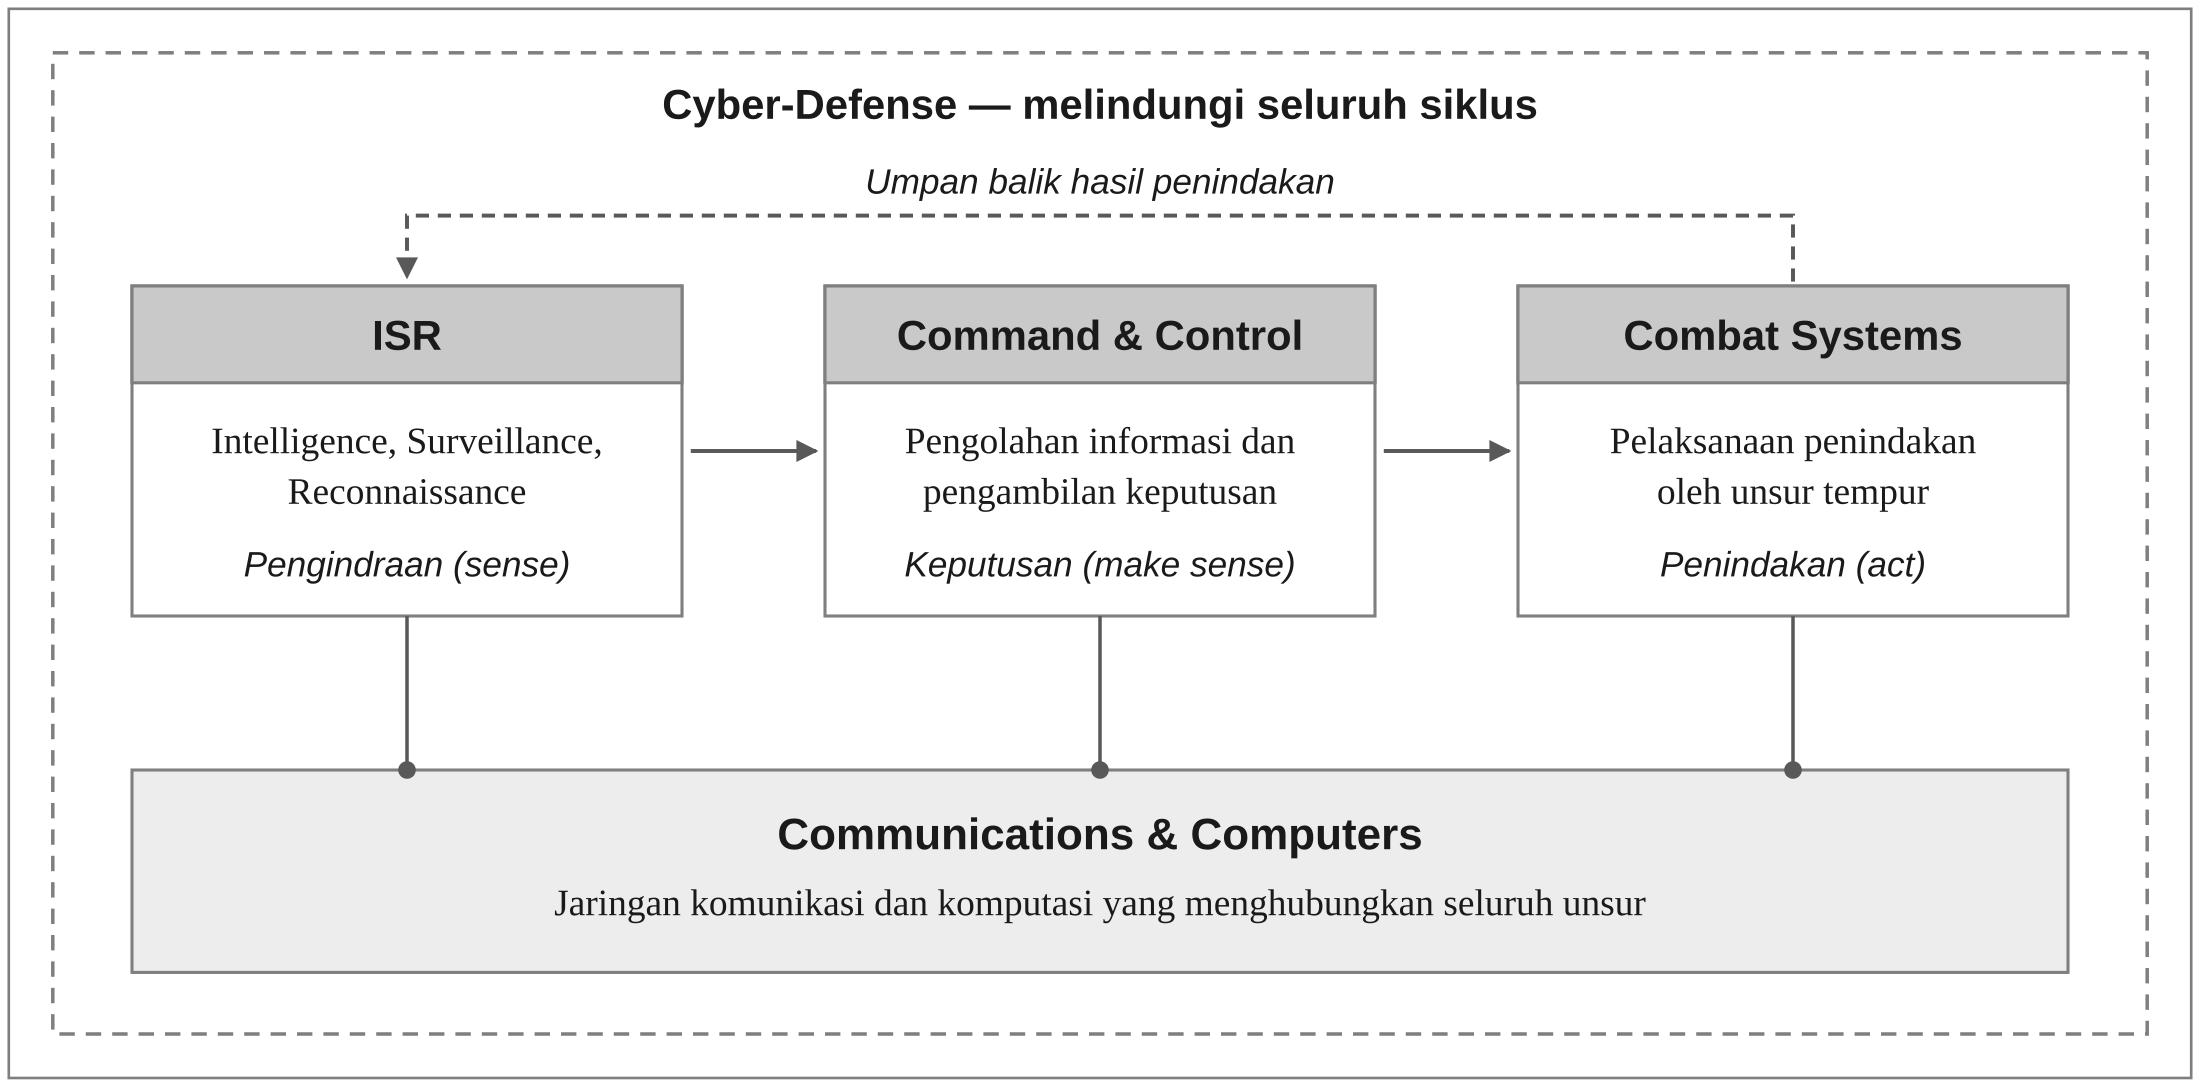
\includegraphics[width=1.00\linewidth,height=0.8\textheight,keepaspectratio]{images/Model Konseptual Keterpaduan Unsur C6ISR.png}
\caption{Model Konseptual Keterpaduan Unsur C6ISR}
\label{fig:II.17}
\end{figure}

Gambar~\ref{fig:II.17} menunjukkan bahwa unsur ISR berperan sebagai pengindraan (\textit{sense}), unsur komando dan kendali mengolah informasi menjadi keputusan (\textit{make sense}), dan \textit{combat systems} melaksanakan penindakan (\textit{act}) yang hasilnya menjadi umpan balik bagi pengindraan berikutnya \cite{USDoD2022}. \textit{Communications} dan \textit{computers} menjadi tulang punggung yang menghubungkan ketiga unsur tersebut, sedangkan \textit{cyber-defense} melindungi seluruh siklus. Karena efektivitas operasi ditentukan oleh keterpaduan antarunsur, keterpaduan tersebut perlu dinyatakan secara eksplisit dalam arsitektur referensi, misalnya melalui model kapabilitas dan pola lintas domain, bukan dengan memecah unsur C6ISR secara terpisah ke setiap domain arsitektur.

Integrasi \textit{combat systems} juga menuntut pengendalian penggunaan kekuatan yang jelas. Kebijakan Departemen Pertahanan Amerika Serikat mensyaratkan sistem senjata otonom dan semi-otonom dirancang agar komandan dan operator tetap dapat menerapkan pertimbangan manusia yang memadai dalam penggunaan kekuatan \cite{DoDD300009}. Prinsip tersebut relevan karena otomasi dan kecerdasan buatan dapat mempercepat keputusan, tetapi tidak menghilangkan tanggung jawab manusia dalam keputusan penindakan.

\subsection{C6ISR dalam Konteks Pertahanan Indonesia}
\label{sec:II.7.4}

Di Indonesia, konsep yang serupa dengan C4ISR telah dikenal dengan istilah K4IPP. Permenhan Nomor 8 Tahun 2016 mendefinisikan K4IPP sebagai sistem yang memadukan unsur komando, kendali, komunikasi, komputerisasi, informasi, pengamatan, dan pengintaian guna meningkatkan kualitas komando dan pengendalian pimpinan kepada unsur pelaksana maupun sistem senjata secara cepat dan tepat. Peraturan tersebut juga membagi penyelenggaraan sistem komunikasi menjadi tingkat Kemhan, sistem komunikasi strategis oleh Mabes TNI, dan sistem komunikasi taktis oleh setiap angkatan \cite{Permenhan8Tahun2016}.

Istilah C6ISR juga telah digunakan dalam kajian di lingkungan Kemhan RI. Kajian Ditjen\label{sk:Ditjen} Pothan\label{sk:Pothan} Kemhan menyebutkan bahwa pembentukan holding BUMN\label{sk:BUMN} industri pertahanan diharapkan mampu mengintegrasikan C6ISR pada tiga matra TNI dalam penerapan \textit{network centric warfare}, serta mengidentifikasi ketergantungan pada satelit sebagai tantangan \cite{Dwipratama2023}. Pada unsur \textit{cyber-defense}, Pedoman Pertahanan Siber mengidentifikasi ancaman terhadap perangkat keras, perangkat lunak, serta data dan informasi pertahanan \cite{Permenhan82Tahun2014}.

Uraian tersebut menunjukkan tiga hal. Pertama, unsur-unsur C6ISR telah memiliki landasan dalam regulasi dan kajian pertahanan Indonesia. Kedua, penyelenggaraannya masih terbagi per tingkat dan per matra, sejalan dengan permasalahan \textit{silo} pada lapisan operasional. Ketiga, C6ISR di Indonesia masih berupa konsep dan istilah, belum dirumuskan sebagai arsitektur referensi yang menautkan kebijakan Kemhan RI dengan kebutuhan operasional TNI. Dalam penelitian ini, C6ISR dirumuskan dari sudut pandang Kemhan RI sebagai penyusun kebijakan dan standar, sedangkan komando dan pengendalian operasional tetap berada pada Mabes TNI.

\section{Penelitian Terkait}
\label{sec:II.8}

Subbab ini menguraikan tiga kelompok penelitian terkait, yaitu EA di sektor pertahanan, arsitektur dan model referensi di sektor pertahanan, serta pengembangan arsitektur referensi untuk domain khusus. Ketiga kelompok tersebut kemudian dibandingkan untuk merumuskan kesenjangan, posisi, dan kebaruan penelitian ini.

\subsection{Enterprise Architecture di Sektor Pertahanan}
\label{sec:II.8.1}

Sejumlah penelitian memadukan \textit{framework} pertahanan dengan TOGAF. Dandashi dkk. menyatakan bahwa TOGAF dan DoDAF saling melengkapi karena TOGAF berfokus pada metode pengembangan, sedangkan DoDAF berfokus pada deskripsi arsitektur, sehingga setiap produk DoDAF dapat dipetakan ke fase ADM \cite{Dandashi2006}. Jørgensen dkk. melaporkan bahwa Angkatan Bersenjata Norwegia menggunakan TOGAF sebagai metode dan NAF sebagai metamodel dan struktur konten, melalui pemetaan rinci antara kerangka konten TOGAF dan NAF, DoDAF, serta MODAF \cite{Jorgensen2011}.

Penelitian lain menerapkan \textit{framework} pertahanan pada objek yang lebih spesifik. Zain dkk. menggunakan DoDAF untuk merancang arsitektur \textit{as-is} dan \textit{to-be} pada sebuah perusahaan industri pertahanan Malaysia dengan penguatan keamanan siber \cite{Zain2023}. Fang dkk. memadukan pola keputusan dengan pemodelan DoDAF untuk menghasilkan alternatif arsitektur \textit{system of systems} pada sistem peperangan antikapal selam \cite{Fang2024}. Lundberg dkk. memperluas NAF dengan tujuh \textit{method chunk} untuk memandu pemodelan sistem C2, yang didemonstrasikan pada integrasi kapabilitas ISR ke dalam sistem C2 \cite{Lundberg2026}.

Penelitian-penelitian tersebut menunjukkan dua pola. Pertama, TOGAF telah digunakan di sektor pertahanan sebagai metode yang dipadukan dengan \textit{framework} pertahanan melalui pemetaan artefak dan metamodel. Kedua, penelitian yang memuat kapabilitas C2 dan ISR dilakukan pada tingkat sistem, bukan pada tingkat EA kementerian.

\subsection{Arsitektur dan Model Referensi di Sektor Pertahanan}
\label{sec:II.8.2}

Pada tingkat aliansi, NATO menggunakan C3 \textit{Taxonomy} sebagai model yang merepresentasikan konsep dan hubungan antarkonsep dalam seluruh siklus hidup kapabilitas \textit{Consultation, Command and Control} (C3) NATO, sekaligus sebagai bahasa bersama yang menghubungkan \textit{Strategic Concept} NATO dengan proses perencanaan pertahanannya \cite{NATOC3Taxonomy}. Standar interoperabilitas NATO juga disusun mengikuti struktur C3 \textit{Taxonomy} \cite{NATONISP}. Dengan demikian, C3 \textit{Taxonomy} berperan sebagai model referensi kapabilitas yang disusun untuk proses perencanaan NATO.

Di Amerika Serikat, Departemen Pertahanan menetapkan lima komponen arsitektur referensi sebagai pedoman penyusunan arsitektur referensi di lingkungannya \cite{DoDCIO2010RA}. Pedoman \textit{Business Enterprise Architecture} tahun 2026 juga menetapkan model tiga lapis, yaitu CIO\label{sk:CIO} menetapkan standar dan model referensi \textit{enterprise} yang otoritatif sebagai acuan arsitektur di bawahnya \cite{DoWBEA2026}. Praktik tersebut menunjukkan bahwa arsitektur referensi digunakan sebagai instrumen kebijakan kementerian pertahanan.

Di Singapura, \textit{Defence Science and Technology Agency} (DSTA\label{sk:DSTA}) mengembangkan \textit{Reference Architecture Framework} untuk mengelola interoperabilitas \textit{system of systems}. \textit{Framework} tersebut membagi permasalahan ke dalam beberapa subdomain yang masing-masing memiliki arsitektur referensi, kemudian dipadukan melalui arsitektur menyeluruh. DSTA juga mengembangkan arsitektur referensi C2 \textit{non-real-time} berbasis SOA dengan desain tiga tingkat \cite{Chang2009}.

Uraian tersebut menunjukkan bahwa arsitektur dan model referensi pertahanan telah digunakan, tetapi disusun untuk proses aliansi atau negara tertentu dan sebagian berada pada tingkat taksonomi kapabilitas atau solusi sistem. Sejauh penelusuran penelitian ini, belum ditemukan arsitektur referensi pertahanan pada tingkat \textit{enterprise} yang mencakup empat domain EA dan selaras dengan regulasi Indonesia.

\subsection{Pengembangan Arsitektur Referensi untuk Domain Khusus}
\label{sec:II.8.3}

Di luar sektor pertahanan, arsitektur referensi sektoral telah digunakan bersama TOGAF ADM. Selain CSPA pada sektor statistik \cite{UNECECSPA2014}, BPS\label{sk:BPS} mengadopsi TOGAF ADM yang disederhanakan menjadi lima tahap dan menggunakan GAMSO\label{sk:GAMSO} serta CSPA sebagai arsitektur rujukan statistik \cite{Virantina2020}. Pada sektor teknologi informasi pemerintahan, NIST\label{sk:NIST} menerbitkan arsitektur referensi komputasi awan yang netral terhadap vendor, yang mendefinisikan lima aktor utama beserta aktivitas dan fungsinya \cite{NISTCCRA2011}.

Pendekatan lain menanamkan muatan domain dengan memodifikasi TOGAF. Setyadi memodifikasi langkah dan artefak ADM untuk membangun \textit{architecture framework} e-government pada pemerintah kabupaten/kota dengan Pemeringkatan e-Government Indonesia sebagai tolok ukur \cite{Setyadi2015}. Bastidas dkk. menemukan bahwa TOGAF belum memuat prinsip, pemangku kepentingan, dan konsep domain \textit{smart city}, sehingga merekomendasikan perluasan ADM dan metamodelnya \cite{Bastidas2023}.

Penelitian-penelitian tersebut menunjukkan dua pola. Pola pertama memodifikasi ADM agar memuat konsep domain. Pola kedua mempertahankan ADM dan menyediakan muatan domain melalui arsitektur referensi sektoral, seperti BPS dengan CSPA. Pola kedua membuat muatan domain dapat digunakan ulang oleh banyak organisasi tanpa mengubah metode. Penelitian ini mengikuti pola kedua untuk sektor pertahanan.

\subsection{Kesenjangan Penelitian}
\label{sec:II.8.4}

Penelitian terkait dibandingkan berdasarkan enam kriteria, yaitu K1 objek pada sektor pertahanan, K2 menggunakan atau menghasilkan arsitektur referensi, K3 memuat kapabilitas operasional pertahanan (C2, ISR, atau C6ISR), K4 mencakup domain bisnis, data, aplikasi, dan teknologi, K5 terintegrasi dengan TOGAF ADM, serta K6 berada dalam konteks regulasi Indonesia. Hasil perbandingan disajikan pada Tabel~\ref{tab:II.10}.

\begingroup\small\setstretch{1.0}
\begin{longtable}{@{}>{\raggedright\arraybackslash\hspace{0pt}}p{0.213\linewidth}>{\raggedright\arraybackslash\hspace{0pt}}p{0.158\linewidth}>{\raggedright\arraybackslash\hspace{0pt}}p{0.069\linewidth}>{\raggedright\arraybackslash\hspace{0pt}}p{0.069\linewidth}>{\raggedright\arraybackslash\hspace{0pt}}p{0.069\linewidth}>{\raggedright\arraybackslash\hspace{0pt}}p{0.069\linewidth}>{\raggedright\arraybackslash\hspace{0pt}}p{0.069\linewidth}>{\raggedright\arraybackslash\hspace{0pt}}p{0.069\linewidth}@{}}
\caption{Pemetaan Penelitian Terkait}\label{tab:II.10}\\
\toprule
\textbf{Penelitian} & \textbf{Objek/Domain} & \textbf{K1} & \textbf{K2} & \textbf{K3} & \textbf{K4} & \textbf{K5} & \textbf{K6}\\
\midrule
\endfirsthead
\multicolumn{8}{@{}l}{\small\itshape \tablename\ \thetable{} (lanjutan)}\\
\toprule
\textbf{Penelitian} & \textbf{Objek/Domain} & \textbf{K1} & \textbf{K2} & \textbf{K3} & \textbf{K4} & \textbf{K5} & \textbf{K6}\\
\midrule
\endhead
\bottomrule
\endlastfoot
\textcite{Dandashi2006} & Pertahanan AS\label{sk:AS} & \centering\arraybackslash √ & \centering\arraybackslash – & \centering\arraybackslash – & \centering\arraybackslash √ & \centering\arraybackslash √ & \centering\arraybackslash –\\*
\textcite{Jorgensen2011} & Angkatan Bersenjata Norwegia & \centering\arraybackslash √ & \centering\arraybackslash – & \centering\arraybackslash – & \centering\arraybackslash √ & \centering\arraybackslash √ & \centering\arraybackslash –\\
\textcite{Zain2023} & Industri pertahanan Malaysia & \centering\arraybackslash √ & \centering\arraybackslash – & \centering\arraybackslash – & \centering\arraybackslash (√) & \centering\arraybackslash – & \centering\arraybackslash –\\
\textcite{Fang2024} & \textit{System of systems} pertahanan & \centering\arraybackslash √ & \centering\arraybackslash – & \centering\arraybackslash (√) & \centering\arraybackslash – & \centering\arraybackslash – & \centering\arraybackslash –\\
\textcite{Lundberg2026} & Sistem C2 & \centering\arraybackslash √ & \centering\arraybackslash – & \centering\arraybackslash √ & \centering\arraybackslash – & \centering\arraybackslash – & \centering\arraybackslash –\\
NATO C3 \textit{Taxonomy} \cite{NATOC3Taxonomy} & Kapabilitas C3 NATO & \centering\arraybackslash √ & \centering\arraybackslash (√) & \centering\arraybackslash √ & \centering\arraybackslash (√) & \centering\arraybackslash – & \centering\arraybackslash –\\
\textcite{Chang2009} & Pertahanan Singapura & \centering\arraybackslash √ & \centering\arraybackslash √ & \centering\arraybackslash √ & \centering\arraybackslash (√) & \centering\arraybackslash – & \centering\arraybackslash –\\
UNECE (2014) \cite{UNECECSPA2014} & Statistik resmi & \centering\arraybackslash – & \centering\arraybackslash √ & \centering\arraybackslash – & \centering\arraybackslash √ & \centering\arraybackslash – & \centering\arraybackslash –\\
\textcite{Virantina2020} & Statistik (BPS) & \centering\arraybackslash – & \centering\arraybackslash √ & \centering\arraybackslash – & \centering\arraybackslash √ & \centering\arraybackslash √ & \centering\arraybackslash √\\
\textcite{Setyadi2015} & E-government kabupaten/kota & \centering\arraybackslash – & \centering\arraybackslash – & \centering\arraybackslash – & \centering\arraybackslash √ & \centering\arraybackslash √ & \centering\arraybackslash √\\
\textcite{Bastidas2023} & \textit{Smart city} & \centering\arraybackslash – & \centering\arraybackslash – & \centering\arraybackslash – & \centering\arraybackslash √ & \centering\arraybackslash (√) & \centering\arraybackslash –\\*
\textbf{Penelitian ini} & \textbf{Pertahanan Indonesia} & \centering\arraybackslash \textbf{√} & \centering\arraybackslash \textbf{√} & \centering\arraybackslash \textbf{√} & \centering\arraybackslash \textbf{√} & \centering\arraybackslash \textbf{√} & \centering\arraybackslash \textbf{√}\\
\end{longtable}
\endgroup

Keterangan: √ = terpenuhi; (√) = terpenuhi sebagian; – = tidak terpenuhi. Tabel~\ref{tab:II.10} menunjukkan bahwa belum terdapat penelitian yang memenuhi keenam kriteria secara bersamaan. Kesenjangan penelitian yang teridentifikasi adalah sebagai berikut.

\begin{enumerate}[label=\arabic*.]
\item Arsitektur dan model referensi pertahanan yang ada disusun untuk konteks aliansi atau negara lain dan sebagian berada pada tingkat taksonomi kapabilitas atau solusi sistem, sehingga belum menyediakan arsitektur referensi tingkat \textit{enterprise} yang mencakup empat domain EA.
\item Penelitian yang memuat kapabilitas C2 dan ISR berada pada tingkat sistem, dan belum ditemukan perumusan C6ISR menjadi arsitektur referensi.
\item Penggunaan arsitektur referensi sektoral bersama TOGAF ADM telah dilakukan pada sektor statistik Indonesia, tetapi belum pada sektor pertahanan, termasuk panduan penerapannya yang selaras dengan regulasi dan Arsitektur SPBE.
\end{enumerate}

\subsection{Posisi dan Kebaruan Penelitian}
\label{sec:II.8.5}

Berdasarkan kesenjangan tersebut, penelitian ini berada pada irisan EA pertahanan, arsitektur referensi, dan C6ISR. Penelitian ini mengikuti pola penggunaan arsitektur referensi sektoral bersama TOGAF ADM tanpa mengubah struktur fasenya, kemudian menerapkannya pada sektor pertahanan dengan C6ISR sebagai landasan muatan. Kandidat kebaruan penelitian ini adalah sebagai berikut.

\begin{enumerate}[label=\arabic*.]
\item Perumusan C6ISR menjadi arsitektur referensi sektoral pertahanan, yaitu DERA, yang memuat \textit{Capability Reference Model}, arsitektur referensi empat domain, dan pola lintas domain.
\item Penyelarasan arsitektur referensi pertahanan dengan regulasi nasional dan Arsitektur SPBE.
\item Panduan penerapan arsitektur referensi pertahanan dalam TOGAF ADM tanpa menambah fase.
\end{enumerate}

Kebaruan tersebut tidak terletak pada TOGAF, C6ISR, atau DSRM secara terpisah, melainkan pada perpaduan ketiganya dalam bentuk arsitektur referensi sektoral untuk pertahanan Indonesia.
